% =====================================================================
% Paper A+B (merged)
% Closed-form absorbed-power dosimetry on the human body, 1 to 100 GHz:
%   from a local Fresnel identity to a whole-body Cauchy formula.
% Author: Robin Wydaeghe
% Target: IEEE Transactions on Antennas and Propagation
% =====================================================================

\documentclass[journal,twocolumn,10pt]{IEEEtran}

\usepackage[utf8]{inputenc}
\usepackage[T1]{fontenc}
\usepackage{lmodern}
\usepackage{microtype}

\usepackage{amsmath,amssymb,amsthm,mathtools}
\usepackage{bm}

\usepackage{graphicx}
\graphicspath{{figures/}{authors/}}
\usepackage{booktabs}
\usepackage{array}
\usepackage{caption}
\usepackage{subcaption}

\usepackage{cite}
\usepackage{xcolor}
\usepackage{tikz}
\usetikzlibrary{arrows.meta,positioning,calc,fit,backgrounds}
\usepackage{xr-hyper}
\externaldocument{paper_SI}
\usepackage[colorlinks=true,linkcolor=black,citecolor=black,urlcolor=black]{hyperref}
\usepackage{orcidlink}
\usepackage[capitalize]{cleveref}
\usepackage[acronym,nonumberlist,nopostdot,nomain]{glossaries}
% Suppress hyperlinks on \gls expansions so they render as plain black text
% rather than picking up the blue linkcolor from hyperref.
\glsdisablehyper

\newcommand*{\doi}[1]{\href{https://doi.org/#1}{#1}}

\newacronym{APD}{APD}{Absorbed Power Density}
\newacronym{IPD}{IPD}{Incident Power Density}
% [circa:a471a26e-d4cc-4b5f-b18f-f8fa19caf44a:begin]
\newacronym{ACS}{ACS}{Absorption Cross-Section}
% [circa:a471a26e-d4cc-4b5f-b18f-f8fa19caf44a:end]
\newacronym{SAR}{SAR}{Specific Absorption Rate}
\newacronym{psSAR10g}{psSAR$_{10\mathrm{g}}$}{peak-spatial SAR averaged over a 10\,g cube}
\newacronym{FDTD}{FDTD}{Finite-Difference Time-Domain}
\newacronym{ICNIRP}{ICNIRP}{International Commission on Non-Ionizing Radiation Protection}
\newacronym{TM}{TM}{Transverse Magnetic}
\newacronym{TE}{TE}{Transverse Electric}
\newacronym{GPU}{GPU}{Graphics Processing Unit}
\newacronym{GELU}{GELU}{Gaussian Error Linear Unit}
\newacronym{ReLU}{ReLU}{Rectified Linear Unit}
\newacronym{BSA}{BSA}{body surface area}

\theoremstyle{plain}
\newtheorem{theorem}{Theorem}
\newtheorem{proposition}[theorem]{Proposition}
\newtheorem{corollary}[theorem]{Corollary}
\theoremstyle{remark}
\newtheorem{remark}[theorem]{Remark}

\crefname{proposition}{Proposition}{Propositions}
\Crefname{proposition}{Proposition}{Propositions}
\crefname{corollary}{Corollary}{Corollaries}
\Crefname{corollary}{Corollary}{Corollaries}
\crefname{remark}{Remark}{Remarks}
\Crefname{remark}{Remark}{Remarks}

% --- math macros ---
\newcommand{\khat}{\hat{\bm{k}}}
\newcommand{\nhat}{\hat{\bm{n}}}
\newcommand{\rr}{\mathbf{r}}
\newcommand{\EE}{\mathbf{E}}
\newcommand{\IPD}{\mathrm{IPD}}
\newcommand{\APD}{\mathrm{APD}}
\newcommand{\Aab}{A_{\mathrm{ab}}}
\newcommand{\Aperp}{A_\perp}
\newcommand{\Teff}{T_{\mathrm{eff}}}
\newcommand{\Tavg}{T_{\mathrm{avg}}}
\newcommand{\Tbar}{\bar{T}}
\newcommand{\Tlay}{T_{\mathrm{lay}}}
\newcommand{\ntilde}{\tilde{n}}
\newcommand{\diff}{\mathrm{d}}
\newcommand{\pospart}[1]{\left[#1\right]_{+}}
\newcommand{\Vis}{V}
% [circa:ae4bd42e-43e3-46b0-8f9b-dd95e0abb914:begin]
\newcommand{\APDAvg}{\langle\mathrm{APD}\rangle_{1\,/\,4\,\mathrm{cm}^2}}
% [circa:ae4bd42e-43e3-46b0-8f9b-dd95e0abb914:end]
\DeclareMathOperator{\RE}{Re}

% Flowchart output-box colors
\definecolor{outA}{RGB}{216,234,251}
\definecolor{outB}{RGB}{251,234,216}
\definecolor{outC}{RGB}{226,247,217}

% Black censor rectangles over eyes and genitals on Thelonious phantom views.
% Rectangle positions are in normalized image coordinates (0,0)=SW, (1,1)=NE.
% Args: [width]{file}{eyes_LL}{eyes_UR}{gen_LL}{gen_UR}, each corner as "x,y".
\newcommand{\censorphantom}[6][\linewidth]{%
  \begin{tikzpicture}
    \node[anchor=south west, inner sep=0] (img) at (0,0)
      {\includegraphics[width=#1]{#2}};
    \begin{scope}[x={(img.south east)}, y={(img.north west)}]
      \fill[black] (#3) rectangle (#4);
      \fill[black] (#5) rectangle (#6);
    \end{scope}
  \end{tikzpicture}%
}

\begin{document}

% [circa:ffc40868-2cb2-4511-b408-c6e19fa281df:begin]
% [circa:c1b8e5a3-b9e1-4219-8299-2089e36f9fe8:begin]
\title{Closed-Form Absorbed-Power Dosimetry from~1~to~100\,GHz}
% [circa:c1b8e5a3-b9e1-4219-8299-2089e36f9fe8:end]
% [circa:ffc40868-2cb2-4511-b408-c6e19fa281df:end]

\author{Robin~Wydaeghe$^{*}$~\orcidlink{0000-0002-1374-0118},
  Luc~Martens~\orcidlink{0000-0001-9948-9157},~\IEEEmembership{Member,~IEEE},
  G\"unter~Vermeeren~\orcidlink{0000-0002-5309-3808},~\IEEEmembership{Member,~IEEE},
  Emmeric~Tanghe~\orcidlink{0000-0003-0020-6466},~\IEEEmembership{Member,~IEEE},
  and~Wout~Joseph~\orcidlink{0000-0002-8807-0673},~\IEEEmembership{Senior~Member,~IEEE}%
  \thanks{All authors are with the WAVES research group, Department of
  Information Technology, Ghent University--imec, Technologiepark-Zwijnaarde
  126, 9052 Ghent, Belgium.}%
  \thanks{$^{*}$Corresponding author. E-mail: robin.wydaeghe@ugent.be.}}

\markboth{IEEE Transactions on Antennas and Propagation,
Vol.~XX, No.~X, Month~Year}%
{Wydaeghe \MakeLowercase{\textit{et~al.}}: Closed-Form
Absorbed-Power Dosimetry}

\maketitle

% [circa:860c7b26-1400-414d-a361-5c0e373a4be6:begin]
\begin{abstract}
Regulatory dosimetry on the human body relies on Finite-Difference
Time-Domain (FDTD) simulation, which becomes prohibitive at mmWave,
where meshes reach $10^{12}$ cells per plane-wave configuration.
We replace the simulation with a closed form derived from the
surface Fresnel law. Two observations make it possible. First, a
pseudo-Brewster compensation holds the unpolarized Fresnel
transmission within 5.6\% of its normal-incidence value across
$0^\circ$--$75^\circ$ on skin at 28~GHz, placing biological tissue
in the high-index regime of the optical-substrate literature and
collapsing the angular dependence to a scalar. Second, this local
law integrates over a body mesh into a generalized Cauchy formula
that extends the classical convex projected-area identity to
nonconvex absorbers, with the self-shadowing factor realized by an
ambient-occlusion pass. A layered Fabry--P\'erot correction in
subcutaneous fat handles the residual below 6~GHz. The closed form
matches Mie theory on lossy spheres, full polarization-aware Fresnel
on the Thelonious phantom within $1.2\%$ direction-averaged on total absorbed power, Sim4Life FDTD at
5.8~GHz with no fitted parameters, and the dosimetry literature
across 168 volunteers and 5 FDTD phantoms. It holds quantitatively
from 1--100~GHz on whole-body quantities and from 6--100~GHz
pointwise on the surface, reducing whole-body compliance to three
precomputed scalars.
\end{abstract}
% [circa:860c7b26-1400-414d-a361-5c0e373a4be6:end]

\begin{IEEEkeywords}
APD, dosimetry, FDTD, Fresnel transmission, ICNIRP, mmWave, SAR.
\end{IEEEkeywords}

\IEEEpeerreviewmaketitle

% Abstract has already spelled out APD, IPD, and FDTD; suppress glossaries
% first-use expansion so subsequent \gls{APD}/\gls{IPD}/\gls{FDTD} render the
% short form.
\glsunset{APD}\glsunset{IPD}\glsunset{FDTD}


\section{Introduction}\label{sec:introduction}
\IEEEPARstart{W}{ireless} exposure on the human body is regulated
through two basic restrictions in the \gls{ICNIRP} 2020
guidelines~\cite{ICNIRP2020}, IEC/IEEE~63195, and IEEE~C95.1: the
mass-averaged \gls{SAR} below 6~GHz, with peak values evaluated as
\gls{psSAR10g}, and the surface-averaged
\gls{APD} above 6~GHz. Direct evaluation uses
\gls{FDTD} simulation on an anatomical
phantom~\cite{Kodera2024,Diao2024,Wydaeghe2026}. Resolving the submillimeter
absorption layer at ten cells per in-tissue wavelength
sets a cell count of $10^{8}$ at 6~GHz, growing to $10^{12}$ near
100~GHz. A regulatory campaign that covers frequencies, postures, and
incidence directions takes weeks on \gls{GPU} clusters. Whole-body
simulations above 30~GHz become infeasible because computational
resources scale with the fourth power of frequency.

Five partial closed forms exist in the literature, each fitting one
empirical scalar to numerical or experimental data. In a reverberation
chamber, the whole-body absorbed power on a volunteer divided by the
% [circa:a471a26e-d4cc-4b5f-b18f-f8fa19caf44a:begin]
\gls{IPD} is the \gls{ACS} $\sigma_a$ in m$^2$.
% [circa:a471a26e-d4cc-4b5f-b18f-f8fa19caf44a:end]
% [circa:ca8c07fd-613a-43cd-8d30-594ac9979669:begin]
Bamba et~al.~\cite{Bamba2014} divide $\sigma_a$ by phantom
mass and fit an empirical efficiency $\eta(f) \approx 0.50$--$0.56$
across $1.45$--$5.8$~GHz.
% [circa:ca8c07fd-613a-43cd-8d30-594ac9979669:end]
Flintoft et~al.~\cite{Flintoft2014} divide
by $\gamma_s\,\mathrm{BSA}/4$, yielding a normalized cross-section
$\langle Q^a \rangle$, where $\gamma_s$ is the body self-shadowing
factor and $\mathrm{BSA}$ is the \gls{BSA}. They report
$\langle Q^a \rangle \approx 0.41$ from 7--11~GHz on $60$ volunteers.
Zhang~\cite{Zhang2017thesis,ZhangRobinson2020} reports a coefficient
$\xi$ of $0.45$--$0.65$ above 6~GHz on $48$ subjects. Kodera
et~al.~\cite{Kodera2024} fit a transmission coefficient
$T_{\mathrm{tr}}$ that matches FDTD to $5\%$ from $10$--$100$~GHz on
% [circa:b4711191-22da-4118-90ab-e781e6720551:begin]
parametric and anatomical phantoms. Diao~et~al.~\cite{Diao2024}
report a single value of the transmission coefficient,
$T = 0.52$ at 28~GHz, obtained from a full-anatomical FDTD
simulation. Three gaps remain.
% [circa:b4711191-22da-4118-90ab-e781e6720551:end]
First, the empirical scalars are obtained from numerical FDTD
or one-dimensional multilayer
solutions~\cite{Kodera2024,Bamba2014} per phantom and per frequency,
not from a closed-form expression, so they encode geometry,
polarization, and tissue physics in a single number that varies
between studies. Second, no closed form treats
nonconvex bodies, and the self-shadowing factor $\gamma_s$ is set by
hand from surface-area tables. Third, the $3$~GHz dip observed by
Flintoft and Zhang admits a planar multilayer-transmission
interpretation~\cite{Zhang2017thesis} but has not been embedded in a
body-surface integral, so the connection to a closed-form
direction-averaged whole-body identity is missing.

This work closes the three gaps with a single closed form derived
from the surface Fresnel law. First, the angular dependence of the
unpolarized Fresnel transmission collapses to a near-constant scalar
on biological tissue, through a balance between rising
\gls{TM} and falling \gls{TE} channels described
for high-index optical substrates~\cite{Azzam2015}; the empirical
scalars are recovered as boundary values of this collapse. Second,
the geometric local law integrates to a generalized Cauchy
formula~\cite{Cauchy1841} that extends the classical convex
projected-area identity to nonconvex absorbing bodies, with the
self-shadowing factor realized by the ambient-occlusion primitive of
computer graphics~\cite{Zhukov1998,Landis2002,AkenineMoller2018}.
Third, a layered Fabry--P\'erot correction in subcutaneous fat
explains the $3$~GHz dip and matches the slope reported by
Flintoft~\cite{Flintoft2014}.

To the best of the authors' knowledge, the paper makes the following
contributions for the first time.
\begin{enumerate}
  \item A closed-form transmission collapse on lossy biological
  tissue, extending Azzam's lossless optical bound to the IT'IS
  Cole--Cole catalog.
  \item A polarization cancellation theorem stating that the angular
  polarization correction vanishes under any of three conditions:
  circular illumination, random ensemble, or multipath averaging.
  \item A generalized Cauchy formula for nonconvex absorbing bodies,
  identifying the exposure factor with the ambient-occlusion
  primitive of computer graphics.
  \item A closed-form 10~g cube SAR through the Cauchy projection
  in the thin-skin regime and through Chew recursion of the
  standing-wave SAR in the layered regime, with a subsurface peak
  criterion for the latter.
  \item A single-equation match across $168$ volunteers and $5$ FDTD
  phantoms from 1--100~GHz, the broadest empirical comparison
  of a closed-form dosimetry prediction reported to date.
\end{enumerate}

The result is a pair of closed forms. The local form gives the
\gls{APD} at a body surface point as the product of the
\gls{IPD}, the Fresnel transmission at normal incidence,
the binary self-shadowing visibility, and the positive part of the
cosine between the surface normal and the wave direction. The
whole-body form gives the direction-averaged absorbed power as the
\gls{IPD} times a flux-weighted Fresnel transmission
times one quarter of the body absorption area. The flux-weighted
transmission reduces to a single quadrature against the IT'IS
Cole--Cole data~\cite{ITISv5,Gabriel1996}, and the absorption area
to a single ambient-occlusion pass on the body mesh.

The empirical scalars in the literature reduce to specific
quantities in the closed forms. The Kodera transmission coefficient
$T_{\mathrm{tr}}$ is the normal-incidence Fresnel transmission $T_0$,
with its near-constancy across angle and polarization explained by
pseudo-Brewster compensation. The Flintoft self-shadowing factor
$\gamma_s$ is the area-weighted mean of the exposure fraction
$\eta(\rr)$. The Bamba efficiency $\eta(f)$ is the flux-weighted
transmission $\Tbar(f)$. The $3$~GHz dip is a Fabry--P\'erot
resonance in fat. The pair holds quantitatively from $1$--$100$~GHz
on whole-body absorbed power and from $6$--$100$~GHz pointwise on
the surface. Below $6$~GHz the layered correction takes over;
\cref{sec:disc} states the regime of validity in detail.
% [circa:d1f32785-5276-4e78-9337-82c7c08dff8f:begin]
Validation runs against three independent volunteer campaigns
(Bamba, Flintoft, Zhang), two FDTD campaigns (Diao, Kodera), and a
new Sim4Life ground truth on the Thelonious phantom.
% [circa:d1f32785-5276-4e78-9337-82c7c08dff8f:end]

% [circa:bdf18b84-729d-418e-903d-09c8cd3f8391:begin]
% [circa:539e5233-c2c3-4e4c-85cb-0ee6a49e4a9c:begin]
\Cref{fig:flowchart} shows the flowchart of our approach: an exact law, three
reductions to a whole-body identity, and three regulatory outputs. The
% [circa:539e5233-c2c3-4e4c-85cb-0ee6a49e4a9c:end]
paper is organized as follows. \Cref{sec:law} derives the exact
polarization-aware absorption law. \Cref{sec:pB} quantifies the
pseudo-Brewster compensation across angle, frequency, and tissue, and
arrives at the geometric local law. \Cref{sec:cauchy} states and proves
the generalized Cauchy formula and treats the layered Fabry--P\'erot
% [circa:28e92f05-5978-4a23-aecb-56064194ca27:begin]
correction below 6~GHz. \Cref{sec:val} compares the closed forms
% [circa:28e92f05-5978-4a23-aecb-56064194ca27:end]
against four independent ground truths. \Cref{sec:corrections} treats
higher-order corrections. \Cref{sec:compliance} reduces whole-body
compliance to three precomputed scalars and gives the cube SAR
corollary. \Cref{sec:disc} states the regime of validity
quantitatively.
% [circa:bdf18b84-729d-418e-903d-09c8cd3f8391:end]

\begin{figure}[!t]
  \centering
% [circa:6e079f08-610d-4e59-a36b-7b2fda2dd407:begin]
  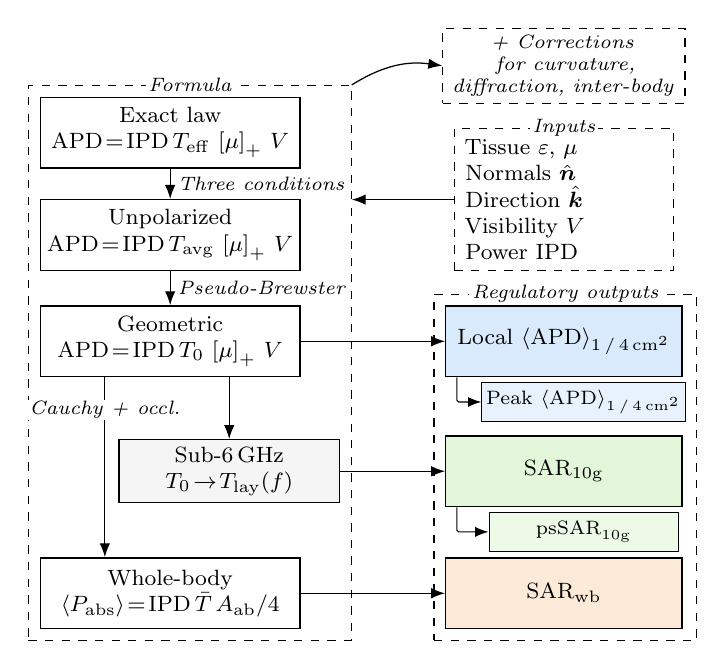
\begin{tikzpicture}[
    every node/.style={font=\footnotesize},
    box/.style={draw=black, line width=0.5pt, rectangle,
                inner sep=2pt, minimum height=9mm, minimum width=33mm,
                fill=white, align=center, font=\footnotesize},
    % [circa:28e92f05-5978-4a23-aecb-56064194ca27:begin]
    sub6/.style={draw=black, line width=0.5pt, rectangle,
                inner sep=2pt, minimum height=8mm, minimum width=28mm,
                fill=black!4, align=center, font=\footnotesize},
    % [circa:28e92f05-5978-4a23-aecb-56064194ca27:end]
    outbox/.style={draw=black, line width=0.5pt, rectangle,
                inner sep=2pt, minimum height=9mm, minimum width=30mm,
                align=center, font=\footnotesize},
    smallout/.style={draw=black, line width=0.4pt, rectangle,
                inner sep=1.5pt, minimum height=5mm, minimum width=24mm,
                align=center, font=\scriptsize},
    inputs/.style={draw=black, line width=0.4pt, rectangle, dashed,
                inner sep=4pt, text width=25mm, align=left,
                font=\footnotesize, fill=white},
    corrbox/.style={draw=black, line width=0.4pt, rectangle, dashed,
                inner sep=2.5pt, text width=29mm, align=center,
                font=\scriptsize\itshape, fill=white},
    arrow/.style={->, line width=0.45pt, >=Latex},
    smallarrow/.style={->, line width=0.4pt, >=Latex,
                rounded corners=0.6pt},
    tag/.style={font=\scriptsize\itshape, align=center,
                fill=white, inner sep=0.6pt}
  ]
% [circa:6e079f08-610d-4e59-a36b-7b2fda2dd407:end]
    % Spine
% [circa:9f017a51-b61f-4165-b8c7-2ac89d7e1c8b:begin]
    \node[box] (exact) at (1.5, 0)     {Exact law\\$\APD\!=\!\IPD\,T_{\mathrm{eff}}\,\pospart{\mu}\,\Vis$};
    \node[box] (avg)   at (1.5, -1.30) {Unpolarized\\$\APD\!=\!\IPD\,\Tavg\,\pospart{\mu}\,\Vis$};
    \node[box] (geom)  at (1.5, -2.65) {Geometric\\$\APD\!=\!\IPD\,T_0\,\pospart{\mu}\,\Vis$};
% [circa:9f017a51-b61f-4165-b8c7-2ac89d7e1c8b:end]
    \node[box] (whole) at (1.5, -5.85) {Whole-body\\$\langle P_{\mathrm{abs}}\rangle\!=\!\IPD\,\Tbar\,\Aab/4$};

    % [circa:28e92f05-5978-4a23-aecb-56064194ca27:begin]
    % Sub-6 GHz inside Formula
% [circa:dd82ebb3-cc32-4bde-9a69-700a963e17cc:begin]
    \node[sub6] (layered) at (2.25, -4.30) {Sub-6\,GHz\\$T_0\!\to\!\Tlay(f)$};
% [circa:dd82ebb3-cc32-4bde-9a69-700a963e17cc:end]
    % [circa:28e92f05-5978-4a23-aecb-56064194ca27:end]

    % Outputs
    \node[outbox, fill=outA] (outLocal) at (6.5, -2.65) {Local $\APDAvg$};
    \node[smallout, fill=outA!60] (outLocalPeak) at (6.75, -3.42) {Peak $\APDAvg$};
% [circa:76ef57d6-7248-4a86-9b2d-934307b0bc4c:begin]
    \node[outbox, fill=outC] (outCube) at (6.5, -4.30) {$\mathrm{SAR}_{10\mathrm{g}}$};
    \node[smallout, fill=outC!60] (outCubePeak) at (6.75, -5.07) {$\mathrm{psSAR}_{10\mathrm{g}}$};
% [circa:76ef57d6-7248-4a86-9b2d-934307b0bc4c:end]
    \node[outbox, fill=outB] (outWB) at (6.5, -5.85) {$\mathrm{SAR}_{\mathrm{wb}}$};

    % Spine arrows top three
    \draw[arrow] (exact) -- node[tag,right=2pt] {Three conditions} (avg);
    \draw[arrow] (avg)   -- node[tag,right=2pt] {Pseudo-Brewster}   (geom);

    % Geom -> Whole at 1/4 width
    \coordinate (geom_q1) at ($(geom.south west)!0.25!(geom.south east)$);
    \coordinate (whole_q1) at ($(whole.north west)!0.25!(whole.north east)$);
% [circa:ed4b8990-3eb2-4bdd-8fdc-d0eb00456444:begin]
    \draw[arrow] (geom_q1) -- node[tag,pos=0.18] {Cauchy + occl.} (whole_q1);
% [circa:ed4b8990-3eb2-4bdd-8fdc-d0eb00456444:end]

% [circa:a507effe-938d-4dd2-906c-364997bbef7d:begin]
    % [circa:28e92f05-5978-4a23-aecb-56064194ca27:begin]
    % Geom -> Sub-6 GHz, drawn straight vertically above the Sub-6 GHz box
    % [circa:28e92f05-5978-4a23-aecb-56064194ca27:end]
    \draw[arrow] (geom.south -| layered.north) -- (layered.north);
% [circa:a507effe-938d-4dd2-906c-364997bbef7d:end]

    % Horizontal east-west arrows
    \draw[arrow] (geom.east)    -- (outLocal.west);
    \draw[arrow] (layered.east) -- (outCube.west);
    \draw[arrow] (whole.east)   -- (outWB.west);

    % Elbow refinement arrows
    \draw[smallarrow] ($(outLocal.south west) + (1.5mm,0)$) |- (outLocalPeak.west);
    \draw[smallarrow] ($(outCube.south west)  + (1.5mm,0)$) |- (outCubePeak.west);

% [circa:6e079f08-610d-4e59-a36b-7b2fda2dd407:begin]
    % Formula and Outputs dashed groups
    \begin{pgfonlayer}{background}
      \node[draw=black, line width=0.4pt, dashed,
            fit=(exact)(whole)(layered),
            inner sep=4pt,
            name=formulabox,
            label={[font=\scriptsize\itshape, anchor=center, fill=white, inner sep=1pt]north:Formula}] {};
      \node[draw=black, line width=0.4pt, dashed,
            fit=(outLocal)(outLocalPeak)(outCube)(outCubePeak)(outWB),
            inner sep=4pt,
            label={[font=\scriptsize\itshape, anchor=center, fill=white, inner sep=1pt]north:Regulatory outputs}] {};
    \end{pgfonlayer}

    % Inputs box
    \node[inputs, label={[font=\scriptsize\itshape, anchor=center, fill=white, inner sep=1pt]north:Inputs}] (inp) at (6.5, -0.85) {%
% [circa:6e079f08-610d-4e59-a36b-7b2fda2dd407:end]
      Tissue $\varepsilon$, $\mu$\\
      Normals $\nhat$\\
      Direction $\khat$\\
      Visibility $\Vis$\\
      Power $\IPD$};

    % Inputs -> Formula
    \draw[arrow] (inp.west) -- (formulabox.east |- inp);

    % Corrections box and curved arrow
    \node[corrbox] (corr) at (6.5, 0.85)
% [circa:7fd7c9f9-cace-4d86-9fdb-180bc09aa4b9:begin]
      {+ Corrections for curvature,\\diffraction, inter-body};
% [circa:7fd7c9f9-cace-4d86-9fdb-180bc09aa4b9:end]
    \draw[arrow] (formulabox.north east) to[bend left=20] (corr.west);
  \end{tikzpicture}
  % [circa:539e5233-c2c3-4e4c-85cb-0ee6a49e4a9c:begin]
  \caption{Flowchart of our approach. The formula has five inputs. Three
  % [circa:539e5233-c2c3-4e4c-85cb-0ee6a49e4a9c:end]
  reductions take the exact law to a whole-body identity. Each arrow
  is one reduction, justified in
  % [circa:28e92f05-5978-4a23-aecb-56064194ca27:begin]
  \cref{subsec:exact-law,sec:pB,subsec:cauchy-thm}. A sub-6~GHz
  branch replaces $T_0$ with a layered transmission $\Tlay(f)$
  % [circa:28e92f05-5978-4a23-aecb-56064194ca27:end]
  (\cref{subsec:fp}). Higher-order corrections are bounded errors on
  the chain (\cref{sec:corrections}). The chain has three regulatory
  % [circa:ae4bd42e-43e3-46b0-8f9b-dd95e0abb914:begin]
  outputs: the surface-averaged \gls{APD} (over $4$~cm$^2$ below 30~GHz,
  $1$~cm$^2$ above), the 10~g cube \gls{SAR},
  % [circa:ae4bd42e-43e3-46b0-8f9b-dd95e0abb914:end]
  and the whole-body \gls{SAR}. Smaller boxes are the peak versions used
  by the \gls{ICNIRP} (\cref{sec:compliance}).}
  \label{fig:flowchart}
\end{figure}

% [circa:bdf18b84-729d-418e-903d-09c8cd3f8391:begin]
% (Section roadmap fused into the flowchart-figure intro paragraph above.)
% [circa:bdf18b84-729d-418e-903d-09c8cd3f8391:end]

\begin{figure}[!t]
  \centering
  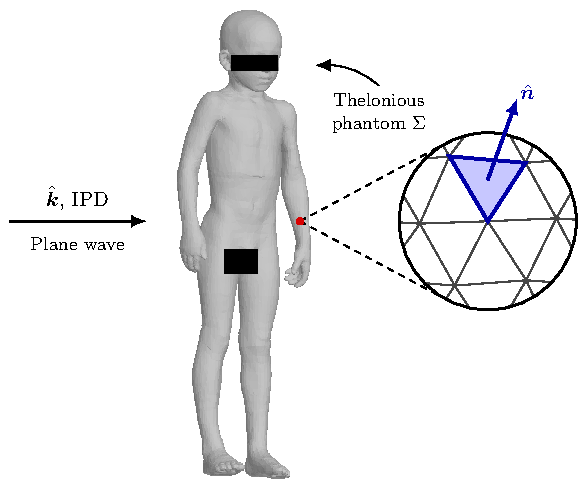
\includegraphics[width=\columnwidth]{fig_geometry.pdf}
  \caption{Configuration of the dosimetry problem. A plane wave with
  intensity $\IPD$ and direction $\hat{\bm{k}}$ illuminates the
  Thelonious phantom. The local \gls{APD} at a visible
  surface point is $\APD = \IPD\,T(\theta)\cos\theta$, with $\theta$
  the angle between $-\hat{\bm{k}}$ and the outward normal
  $\hat{\bm{n}}$ on the triangulated body surface, and $T$ the
  Fresnel transmission.}
  \label{fig:configuration}
\end{figure}


\section{Local absorption law}\label{sec:law}

\Cref{fig:configuration} shows the configuration. A plane wave with
intensity $\IPD$ and direction $\khat$ illuminates the body, and we
evaluate the \gls{APD} $\APD(\rr)$ at every visible
surface point. The derivation below is exact; all approximations are
introduced in subsequent sections.

\subsection{Setup}
A monochromatic plane wave with time-averaged Poynting vector
$\mathbf{S}_{\mathrm{inc}} = \IPD\,\khat$ (units W/m$^2$) illuminates
a body. Three working assumptions hold throughout. First, the
surface $\Sigma$ is locally flat on the wavelength scale. Second, the
skin depth at every frequency of interest is much smaller than any
body dimension, so all power transmitted through the surface is
absorbed within a thin surface layer. Third, coherent reflections
from internal tissue interfaces and from other body parts are
neglected at this stage and re-enter as bounded corrections in
\cref{sec:cauchy,sec:corrections}. At a surface point $\rr$ with
outward unit normal $\nhat(\rr)$, the incidence cosine is
$\mu(\rr) \equiv \nhat(\rr)\cdot(-\khat) = \cos\theta_i(\rr)$. A
front-facing point has $\mu > 0$; a point facing away from the
source has $\mu \le 0$.

\subsection{Power flux through the surface}
The inward power flux through a surface element $\diff A$ at $\rr$
is $\diff P_{\mathrm{in}} = \IPD\,\mu\,\diff A$. The reflected wave
propagates in the specular direction with power density
$|r(\theta_i)|^2\,\IPD$, where $r(\theta_i)$ is the Fresnel amplitude
reflection coefficient appropriate to the polarization. Energy
conservation at a lossy half-space gives
\begin{equation}\label{eq:Sab-pol}
  \APD(\rr) = \IPD \cdot T(\theta_i) \cdot \mu(\rr),
  \qquad T(\theta_i) \equiv 1 - |r(\theta_i)|^2\, ,
\end{equation}
for each polarization separately.

\subsection{Fresnel coefficients}
The body surface is modeled as a planar interface between free
space ($n_1 = 1$) and a lossy medium with complex refractive index
$\ntilde = \sqrt{\varepsilon_r - i\sigma/(\omega\varepsilon_0)}$. The
normal component of the wave vector inside the medium is
$\xi = \sqrt{\ntilde^2 - 1 + \mu^2}$ with $\RE(\xi) > 0$. Continuity
of the tangential fields gives
\begin{equation}\label{eq:rs-rp}
  r_s = \frac{\mu - \xi}{\mu + \xi},
  \qquad
  r_p = \frac{\ntilde^2\,\mu - \xi}{\ntilde^2\,\mu + \xi}\, ,
\end{equation}
for TE and TM polarizations, respectively. The corresponding
power-absorption
coefficients are $T_s(\theta) = 1 - |r_s|^2$ and
$T_p(\theta) = 1 - |r_p|^2$. At normal incidence, $\mu = 1$ and
$\xi = \ntilde$, giving the polarization-degenerate value
\begin{equation}\label{eq:T0}
  T_0 \equiv T_s(0) = T_p(0) = \frac{4\,\RE(\ntilde)}{|1+\ntilde|^2}\, .
\end{equation}
For skin at 28~GHz with $\varepsilon_r = 16.55$ and
$\sigma = 25.8$~S/m, $\ntilde = 4.49 - 1.79i$ and $T_0 = 0.539$.

\subsection{Polarization-aware exact law}\label{subsec:exact-law}
A monochromatic plane wave is fully polarized. At a surface point
$\rr$, decompose the incident electric field into local TE and TM
components by projecting on the unit vectors
$\hat{e}_s(\rr) = \khat \times \nhat / |\khat \times \nhat|$ and
$\hat{e}_p(\rr) = \hat{e}_s \times \khat$. Writing the field as
$\EE_0 = a_s \hat{e}_s + a_p \hat{e}_p$ and the local TE and TM
energy fractions as $|e_s|^2 = |a_s|^2 / |\EE_0|^2$ and
$|e_p|^2 = |a_p|^2 / |\EE_0|^2$, the effective transmission at $\rr$
is
\begin{equation}\label{eq:Teff}
  \Teff(\rr) = |e_s(\rr)|^2 \, T_s(\theta) + |e_p(\rr)|^2 \,
  T_p(\theta)\, .
\end{equation}
The exact \gls{APD} at a visible point is therefore
% [circa:eeba0059-34d6-415a-87c2-5bac3012d008:begin]
\begin{equation}\label{eq:Sab-exact}
  \APD(\rr) = \IPD \, \Teff(\rr) \, \pospart{\mu(\rr)} \,.
\end{equation}
% [circa:eeba0059-34d6-415a-87c2-5bac3012d008:end]
\Cref{eq:Sab-exact} holds for any polarization, any frequency where
the body is opaque, and any locally flat surface. The self-shadowing
factor $\Vis(\rr,\khat)$ of the geometric law in \cref{sec:pB} is
suppressed in this subsection because the Fresnel calculation
operates at a point already taken to be visible. Visibility re-enters
with the multi-source matrix form in \cref{subsec:matrix}.

To proceed, write
\begin{equation}\label{eq:Teff-decomp}
  \Teff(\rr) = \Tavg(\theta) + \tfrac{1}{2}\,q(\rr)\,\Delta T(\theta)\, ,
\end{equation}
with $\Tavg = \tfrac{1}{2}(T_s + T_p)$ the unpolarized baseline,
$\Delta T = T_p - T_s$ the polarization splitting, and $q = |e_p|^2 -
|e_s|^2 \in [-1, 1]$ the local TM excess. The second term vanishes
under any of three conditions. First, for circular polarization the
TE and TM intensities are equal at every point on every body, so
$q \equiv 0$ pointwise. Second, for linear polarization with random
ensemble orientation either in space or time, the ensemble average $\langle q\rangle$
vanishes by the same argument. Third, for a body in a multipath
environment with $N$ independent path orientations, the variance of
the polarization correction scales as $D_B/\sqrt{2N}$, where
$D_B \le 16\%$ is the body's polarization directivity on the
Thelonious phantom; for $N \ge 20$ paths the correction drops below
$2.5\%$. Section~\ref{si:fresnel} of the SI derives all three
conditions and the $D_B/\sqrt{2N}$ variance bound. Under any of these conditions the exact law reduces to
\begin{equation}\label{eq:Sab-Tavg}
  \APD(\rr) = \IPD \, \Tavg(\theta(\rr)) \, \pospart{\mu(\rr)}\, .
\end{equation}
The angular dependence is now confined to the scalar function
$\Tavg(\theta)$. The next section shows that this function is nearly
constant for biological tissue.


\section{Pseudo-Brewster compensation}\label{sec:pB}

The unpolarized Fresnel transmission $\Tavg(\theta)$ is the average
of two angularly opposed quantities. As the incidence angle
increases, $T_s(\theta)$ decreases monotonically, while $T_p(\theta)$
rises toward a near-unity peak at the pseudo-Brewster angle and
then falls. Their average tracks $T_0$ across a wide angular range,
and the angle-dependent factor in~\eqref{eq:Sab-Tavg} reduces to a
scalar at the cost of a few-percent error.

\subsection{Mechanism}\label{subsec:pB-mech}
The Brewster angle of a lossless dielectric is $\theta_{\mathrm{B}} =
\arctan(n_2/n_1)$, at which the TM reflection coefficient
vanishes~\cite{BornWolf1999}. For a lossy dielectric the reflection
minimum is finite but small. The angle at which $|r_p|^2$ is
minimized is the \textit{pseudo-Brewster angle} and satisfies
$\theta_{\mathrm{pB}} \approx \arctan|\ntilde|$ to within $1^\circ$ for
$|\ntilde| > 3$~\cite{Potter1970,Ohman1977}. At this angle, $T_p$
peaks near $0.95$, while $T_s$ has fallen below $0.20$. Their
average $\Tavg(\theta_{\mathrm{pB}}) \approx 0.5$ is close to the
normal-incidence value $T_0 \approx 0.5$--$0.6$ for biological
tissue at mmWave.

Azzam~\cite{Azzam2015} showed that for lossless dielectric substrates
with refractive index $|\ntilde| > 2 + \sqrt{3} \approx 3.73$, the
unpolarized reflectance varies by less than $1\%$ over $[0^\circ,
60^\circ]$. Empirically, the near-constancy extends to $|\ntilde| > 2.5$,
below the strict Azzam threshold. Section~\ref{si:azzam} and
Table~\ref{tab:itis-pB} of the SI evaluate the extension on the
IT'IS v$5.0$ catalog. Biological tissue at the wireless mmWave
band has $|\ntilde| \in [3, 6]$, putting it in the high-index
regime. This connection between the Azzam criterion and biological dosimetry
has not appeared in the optics or bioelectromagnetics literature.

\subsection{Quantitative behavior across angle}\label{subsec:pB-quant}
\Cref{fig:apd-angle} illustrates the compensation for skin at
28~GHz. The upper panel shows $T_s$, $T_p$, and $\Tavg$ versus
incidence angle. The lower panel shows the \gls{APD}
$\APD/\IPD = T(\theta)\cos\theta$ for each polarization and for the
simplified product $T_0\cos\theta$. The unpolarized curve closely
tracks the simplified prediction, and the small gap is the Fresnel
approximation error.

\begin{figure}[!t]
  \centering
  \begin{subfigure}[t]{\columnwidth}
    % [circa:b1cd21c1-256d-4234-bdc0-f5b6cdf82742:begin]
    % In-figure label renamed to "Pseudo-Brewster angle" and shifted left
    % to clear its arrow; see scripts/apd_direction_analysis.py.
    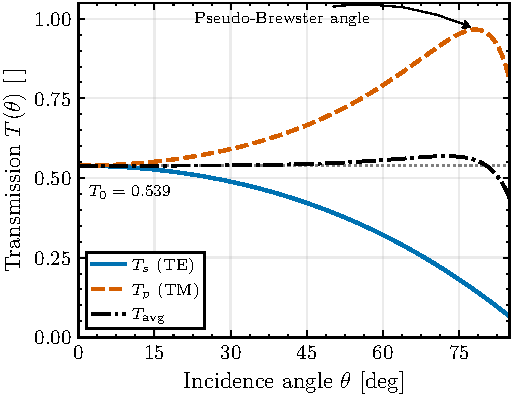
\includegraphics[width=\linewidth]{apd_angle_panel_T.pdf}
    % [circa:b1cd21c1-256d-4234-bdc0-f5b6cdf82742:end]
    \caption{Fresnel transmission $T$.}
    \label{fig:apd-angle:T}
  \end{subfigure}\\[2pt]
  \begin{subfigure}[t]{\columnwidth}
    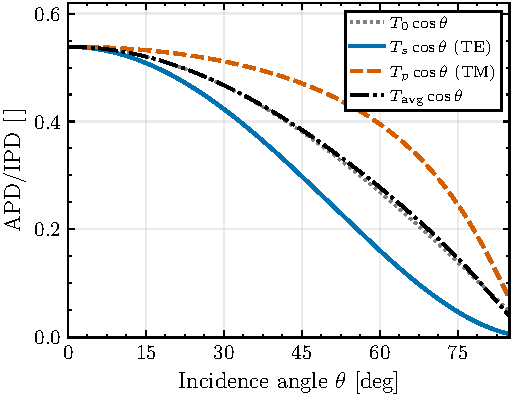
\includegraphics[width=\linewidth]{apd_angle_panel_APD.pdf}
    \caption{Normalized absorbed power $\APD/\IPD$.}
    \label{fig:apd-angle:APD}
  \end{subfigure}
  \caption{Pseudo-Brewster compensation for skin at 28~GHz
  ($\ntilde = 4.49 - 1.79i$, $T_0 = 0.539$). (a)~Fresnel
  power-absorption coefficients $T_s$ (TE), $T_p$ (TM), and
  $\Tavg = \tfrac{1}{2}(T_s + T_p)$ versus incidence angle $\theta$.
  $\Tavg$ stays within $5.6\%$ of $T_0$ up to $75^\circ$.
  (b)~Normalized absorbed power $\APD/\IPD = T(\theta)\cos\theta$
  for the same three states. The dotted reference is the simplified
  $T_0\cos\theta$ prediction.}
  \label{fig:apd-angle}
\end{figure}

\Cref{tab:fresnel-skin} quantifies the deviation of $\Tavg$ from
$T_0$ across $[0^\circ, 75^\circ]$ on skin at 28~GHz. The maximum
is $5.6\%$ at $70$--$75^\circ$. Below $30^\circ$ the agreement
is at the fourth significant figure.

\begin{table}[!t]
\centering
\caption{Fresnel transmission for skin at 28~GHz. The ratio
$\Tavg/T_0$ stays within $5.6\%$ of unity over $[0^\circ,
75^\circ]$.}
\label{tab:fresnel-skin}
\begin{tabular}{ccccc}
\toprule
$\theta$ & $T_s$ (TE) & $T_p$ (TM) & $\Tavg$ & $\Tavg/T_0$ \\
\midrule
$0^\circ$  & 0.539 & 0.539 & 0.539 & 1.000 \\
$30^\circ$ & 0.489 & 0.591 & 0.540 & 1.002 \\
$45^\circ$ & 0.422 & 0.666 & 0.544 & 1.010 \\
$60^\circ$ & 0.321 & 0.791 & 0.556 & 1.032 \\
$70^\circ$ & 0.233 & 0.902 & 0.568 & 1.054 \\
$75^\circ$ & 0.182 & 0.952 & 0.567 & 1.053 \\
\bottomrule
\end{tabular}
\end{table}

\subsection{Tissue universality}\label{subsec:pB-tissues}
All biological tissues at the wireless mmWave band cluster in the
$|\ntilde| > 2.5$ region where the compensation operates.
\Cref{tab:materials} lists the relevant parameters at 28~GHz from
the IT'IS v$5.0$ Cole--Cole model~\cite{ITISv5,Gabriel1996}. Skin and
muscle have $|\ntilde|$ near $5$ and an angular variation below
$5.6\%$. Water has $|\ntilde| > 6$ and a variation below $4\%$.
Fat is the outlier, with $|\ntilde| \approx 2$ and an $8.2\%$
variation, but fat is rarely the outermost tissue at exposure sites
of regulatory interest. Table~\ref{tab:itis-pB} and
Fig.~\ref{fig:si-tissue-universality} of the SI narrow the
evaluation to the three tissues that can be the outermost layer at
exposure surfaces above $6$~GHz: skin, subcutaneous fat, and
vitreous humor. Table~\ref{tab:itis-pB} reports the angular
variation of $\Tavg/T_0$ over $[0^\circ, 60^\circ]$ and $[0^\circ,
75^\circ]$ separately.

\begin{table}[!t]
\centering
\caption{Pseudo-Brewster compensation across tissue types at
28~GHz. The variation column is the maximum deviation of
$\Tavg/T_0$ from unity over $[0^\circ, 75^\circ]$.}
\label{tab:materials}
\begin{tabular}{lccccc}
\toprule
Tissue & $\varepsilon_r$ & $\sigma$\,[S/m] & $|\ntilde|$ & $T_0$
  & $\Tavg$ var. \\
\midrule
Skin   & 17.0 & 25.0 & 4.84 & 0.54 & $5.6\%$ \\
Muscle & 25.0 & 30.0 & 5.62 & 0.48 & $4.8\%$ \\
Fat    &  4.0 &  2.0 & 2.05 & 0.77 & $8.2\%$ \\
Water  & 25.0 & 55.0 & 6.62 & 0.45 & $3.9\%$ \\
\bottomrule
\end{tabular}
\end{table}

\subsection{Frequency dependence}\label{subsec:pB-freq}
The accuracy of the constant-$T_0$ approximation has a clean
frequency dependence. Define the sphere ratio
\begin{equation}\label{eq:R-of-f}
  R(f) \equiv T_0(f) / \Tbar(f),
  \qquad
  \Tbar(f) \equiv 2\int_0^1 \Tavg(\mu, f)\,\mu\,\diff\mu\,,
\end{equation}
where $\Tbar(f)$ is the flux-weighted Fresnel transmission. $R(f) =
1$ when the constant-$T_0$ approximation is exact on a
direction-averaged quantity. $R < 1$ means $T_0$ underestimates
absorbed power. $R > 1$ means it overestimates. \Cref{fig:R-of-f}
shows that for skin the crossover is at 40.4~GHz, where the
compensation is exact to four significant figures. Below this
frequency the approximation is conservative for compliance, in the
sense that it underestimates absorbed power. Above, it overestimates
by at most $3.5\%$ at 100~GHz. The root-mean-square error
remains below $5\%$ across $0.3$--100~GHz. Frequency-resolved
Cole--Cole values for skin and the angle family
$\Tavg(\theta)\cos\theta$ at six representative frequencies are in
Table~\ref{tab:itis-fvs} and Fig.~\ref{fig:si-angle-family} of the SI.

\begin{figure}[!t]
  \centering
  % [circa:04764a12-1ce7-42a6-a270-ffe82b10059a:begin]
  % Legend entries capitalized (Conservative / Non-conservative); see
  % scripts/R_of_f_landscape.py.
  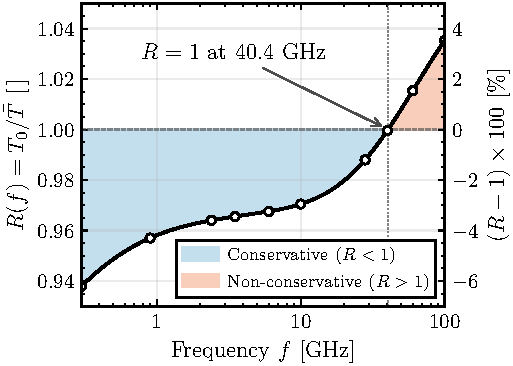
\includegraphics[width=\columnwidth]{R_of_f.pdf}
  % [circa:04764a12-1ce7-42a6-a270-ffe82b10059a:end]
  \caption{Sphere ratio $R(f) = T_0/\Tbar$ versus frequency for skin
  (IT'IS v$5.0$ Cole--Cole model). $R = 1$ indicates that the
  constant-$T_0$ approximation is exact on the direction-averaged
  quantity; $R < 1$ means $T_0$ underestimates absorbed power and
  $R > 1$ means it overestimates. The dashed horizontal lines mark
  the $\pm 4\%$ band.}
  \label{fig:R-of-f}
\end{figure}

\subsection{Geometric absorption law}\label{subsec:pB-geom}
Two simplifications act on the exact law~\eqref{eq:Sab-exact}.
First, we apply the polarization reduction~\eqref{eq:Sab-Tavg}.
Second, we substitute $\Tavg(\theta) \to T_0$ and reinstate
self-shadowing through the binary visibility
$\Vis(\rr,\khat) \in \{0,1\}$. The exact law reduces to the
\textit{geometric absorption law}
% [circa:eeba0059-34d6-415a-87c2-5bac3012d008:begin]
\begin{equation}\label{eq:geom-law}
  \APD(\rr) \approx \IPD \cdot T_0 \cdot \Vis(\rr,\khat) \cdot
  \pospart{\nhat(\rr) \cdot (-\khat)} \, .
\end{equation}
% [circa:eeba0059-34d6-415a-87c2-5bac3012d008:end]
The tissue physics enters through the scalar $T_0$. All spatial
variation depends on the body shape through the surface-normal field
$\nhat(\rr)$ and the visibility field $\Vis(\rr,\khat)$. For a convex
body $\Vis \equiv 1$ and~\eqref{eq:geom-law} reduces to the classical
convex form $\IPD\,T_0 \pospart{\nhat\cdot(-\khat)}$.
\Cref{fig:phantom}\subref{fig:phantom:sab} contrasts the convex-limit prediction with the
visibility-aware result on the Thelonious phantom and motivates the
explicit $\Vis$ factor. Under frontal illumination, the medial
thighs, the inside of the wrists, and the underside of the chin
are the largest self-shadowed regions, and drop to zero through
$\Vis$. The transmission coefficient
$T_{\mathrm{tr}}$ fitted in
\cite{Kodera2024,Diao2024,Funahashi2018} is identified with $T_0$,
and its near-constancy across angle and polarization is the
pseudo-Brewster compensation.

\begin{figure*}[!t]
  \centering
  \begin{subfigure}[b]{0.30\linewidth}
    \centering
    \censorphantom[0.9\linewidth]{sab_phantom_visible.pdf}%
      {0.310,0.880}{0.560,0.915}{0.260,0.440}{0.480,0.490}
    \caption{$\APD(\rr)$, frontal $\khat$.}
    \label{fig:phantom:sab}
  \end{subfigure}\hfill
  \begin{subfigure}[b]{0.30\linewidth}
    \centering
    \censorphantom[0.9\linewidth]{eta_phantom_front.pdf}%
      {0.250,0.870}{0.460,0.905}{0.260,0.440}{0.480,0.490}
    \caption{$\eta(\rr)$, front view.}
    \label{fig:phantom:eta-front}
  \end{subfigure}\hfill
  \begin{subfigure}[b]{0.30\linewidth}
    \centering
    \censorphantom[0.9\linewidth]{eta_phantom_side.pdf}%
      {0.150,0.870}{0.290,0.905}{0.260,0.440}{0.480,0.490}
    \caption{$\eta(\rr)$, side view.}
    \label{fig:phantom:eta-side}
  \end{subfigure}
  % [circa:8e6834c1-7612-4929-95a7-f5f5d4ea84e8:begin]
  \caption{$\APD$ and $\eta$ maps on the Thelonious phantom (skin
  at 28~GHz, $\IPD = 1$~W/m$^2$,
  % [circa:8e6834c1-7612-4929-95a7-f5f5d4ea84e8:end]
  area-weighted mean $\bar\eta = 0.865$). (a)~\Gls{APD}
  under frontal illumination $\khat = +\hat{y}$. Front-facing
  triangles absorb at the cosine rate $T_0\,\IPD\,\cos\theta$.
  Self-shadowed elements drop to zero through $\Vis(\rr,\khat)$.
  (b,~c)~Direction-isotropic exposure fraction
  $\eta(\rr) \in [0,1]$ from~\eqref{eq:eta-def}, front and side
  views. Panel~(a) is the integrand of the Cauchy formula along
  one direction. Panels~(b,~c) integrate over the full sphere.}
  \label{fig:phantom}
\end{figure*}

Hence, the error of~\eqref{eq:geom-law} relative to the exact
polarization-aware law is bounded by the maximum of the polarization
correction and the angular variation of $\Tavg$. The latter is below
$5\%$ across the wireless mmWave band. The former is below
$2.5\%$ for $N \ge 20$ independent multipath components, and at
most $16\%$ on a real human body for the worst-case linearly
polarized single plane wave. The combined error is below the
$20\%$ uncertainty in tissue dielectric properties at
mmWave~\cite{AlekseevZiskin2007}.

\subsection{Discrete multi-source form}\label{subsec:matrix}
Equation~\eqref{eq:geom-law} extends to a triangle mesh under
multiple incident waves. Tile the body by $M$ triangles. Row $j$ of
$\mathbf{N} \in \mathbb{R}^{M\times 3}$ holds the outward unit
normal $\nhat_j$. Let $N$ plane waves arrive with unit directions
$\khat_1, \ldots, \khat_N$ and power densities $S_1, \ldots, S_N$.
Stack the directions column-wise into
$\mathbf{K} \in \mathbb{R}^{3\times N}$, with column $i$ equal to
$-\khat_i$. Stack the powers into
$\mathbf{s} = [S_1,\ldots,S_N]^\top \in \mathbb{R}^N$. Let
$\mathbf{V} \in \{0,1\}^{M\times N}$ be the visibility matrix, with
$V_{ji} = 1$ when direction $\khat_i$ reaches triangle $j$, and
$V_{ji} = 0$ otherwise. Collect the per-triangle APD values into
$\bm{\mathrm{APD}} \in \mathbb{R}^{M}$.

The geometric law on the mesh then reads
\begin{equation}\label{eq:mat-multi}
  \bm{\mathrm{APD}} = T_0\,\bigl(\pospart{\mathbf{N}\,\mathbf{K}}
  \odot \mathbf{V}\bigr)\,\mathbf{s}\, .
\end{equation}
The cosine matrix $\mathbf{N}\,\mathbf{K} \in \mathbb{R}^{M\times N}$
has entry $(j,i)$ equal to $\nhat_j\cdot(-\khat_i)$. The operator
$\pospart{\cdot} \equiv \max(\cdot,0)$ acts componentwise, and clamps
back-facing entries to zero. The Hadamard product $\odot$ with
$\mathbf{V}$ gates self-shadowed entries. The product with
$\mathbf{s}$ sums the contributions of the $N$ incident waves.

Each step is differentiable. Replacing $\pospart{\cdot}$ with the
smooth \gls{GELU} activation~\cite{Hendrycks2016} leaves the
structure intact, and replaces the hard cutoff with a soft rolloff
(\cref{eq:gelu}). Gradients of regulatory quantities with respect to
antenna positions, antenna orientations, and RIS phases propagate
through any differentiable ray tracer~\cite{SionnaRT}. The arithmetic
primitive is the per-pixel shading operation that consumer GPUs run
at frame rate, with the cosine gate playing the role of rectified
shading, and $\mathbf{V}$ the role of ambient occlusion. For $M
\approx 10^4$ and $N \approx 10^2$, the spatial map is one
matrix-vector multiply on the GPU.


\section{Whole-body absorbed power}\label{sec:cauchy}

The local law~\eqref{eq:geom-law} integrates over directions and
positions to a closed-form expression for the direction-averaged
whole-body absorbed power. The classical projected-area formula of
Cauchy~\cite{Cauchy1841} is the special case $\eta \equiv 1$,
$\Tbar \equiv T_0$. This step is the third arrow in
\cref{fig:flowchart}.

\subsection{Self-shadowing and ambient occlusion}\label{sec:self-shadow}
The human body is not convex. Concavities such as the armpits, the
gap between the legs, and the neck region cause one part of the body
to shadow another. The binary visibility $\Vis(\rr,\khat) \in \{0,1\}$
in~\eqref{eq:geom-law} is the ambient-occlusion primitive of computer
graphics introduced by Zhukov et~al.~\cite{Zhukov1998} and brought
into production rendering by Landis~\cite{Landis2002}. Modern GPUs
evaluate $\Vis(\rr,\khat)$ at interactive frame
rates~\cite{AkenineMoller2018}.

\begin{remark}[Exposure fraction]\label{rem:eta}
The \textit{exposure fraction} at a surface point $\rr$ is the cosine-weighted
fraction of the upper hemisphere from which $\rr$ is unobstructed,
\begin{equation}\label{eq:eta-def}
  \eta(\rr) = \frac{1}{\pi}\int_{S^2}
  \pospart{\nhat(\rr)\cdot(-\khat)}\,\Vis(\rr,\khat)\,\diff\Omega\, .
\end{equation}
For convex bodies $\Vis \equiv 1$ and $\eta \equiv 1$. For nonconvex
bodies $\eta \in [0,1]$.
\end{remark}

The exposure fraction $\eta$ is mathematically identical to the
self-shadowing factor $\gamma_s$ that Flintoft et~al.\ define as
``the proportion of total surface area of the body that is illuminated
by the reverberant field''~\cite[p.~3301]{Flintoft2014} and estimate
geometrically as $0.75$--$0.85$ from Tomita's surface-area
data~\cite{Tomita1999}. The Flintoft estimate is geometric and
posture-dependent. The construction here is computational and
posture-resolved. For the Thelonious phantom, an ambient-occlusion
solver returns the area-weighted mean
$\bar{\eta} = \Aab/A = 0.865$. This is near the upper end of
Flintoft's band $[0.75, 0.85]$~\cite{Tomita1999}, and is rendered
on the phantom in \cref{fig:phantom}\subref{fig:phantom:eta-front}
and \cref{fig:phantom}\subref{fig:phantom:eta-side}. Most of the
body has $\eta \approx 1$. Reductions occur in concavities. The
medial sides of the legs and arms, the armpits, the underside of
the chin, and the soles of the feet are the dominant such regions.
On a $10^4$--$10^5$ triangle mesh the solver evaluates $\eta$ in
tens of milliseconds on commodity hardware.

\subsection{Generalized Cauchy formula}\label{subsec:cauchy-thm}

\begin{theorem}[Generalized Cauchy formula]\label{thm:cauchy}
Let a body $\Sigma$ have surface area $A$, exposure fraction
$\eta(\rr)$, and absorption area
$\Aab \equiv \int_\Sigma \eta(\rr)\,\diff A$. Under isotropic,
unpolarized plane-wave illumination of intensity $\IPD$ on tissue
with normal-incidence transmission $T_0$, the direction-averaged
whole-body absorbed power is
\begin{equation}\label{eq:cauchy}
  \langle P_{\mathrm{abs}} \rangle = \IPD\,T_0\,\Aab/4\, .
\end{equation}
\end{theorem}

\begin{proof}
Apply Fubini's theorem to exchange the surface and direction
integrals. The local law~\eqref{eq:geom-law} gives
$\APD(\rr,\khat) = \IPD\,T_0\,\Vis(\rr,\khat)\,
\pospart{\nhat\cdot(-\khat)}$. The direction average of the integrand
is
\[
  \frac{1}{4\pi}\int_{S^2}
  \IPD\,T_0\,\Vis(\rr,\khat)\,\pospart{\nhat\cdot(-\khat)}\,
  \diff\Omega
  = \frac{\IPD\,T_0}{4}\,\eta(\rr),
\]
using the definition of $\eta$ and the identity $\int_{S^2}
\pospart{\nhat\cdot(-\khat)}\,\diff\Omega = \pi$ for any unit
$\nhat$. Integration over $\Sigma$ gives~\eqref{eq:cauchy}.
\end{proof}

The classical Cauchy formula $\langle\Aperp\rangle = A/4$ is the
special case $\eta \equiv 1$, valid for any convex body. The
absorption area $\Aab$ reduces all geometric complexity of
self-shadowing to a single scalar.

\begin{remark}[Convex-hull energy bound]\label{rem:hull}
Let $A_{\mathrm{CH}}$ be the surface area of the convex hull of the
body. Energy conservation under isotropic illumination implies
$\langle P_{\mathrm{abs}} \rangle \le \IPD\,A_{\mathrm{CH}}/4$,
because the power entering the convex hull bounds the absorbed power.
For the Thelonious phantom $A_{\mathrm{CH}}/A \approx 1.20$, so the
hull bound brackets the true absorbed power within a few percent.
\end{remark}

The constant-$T_0$ approximation in~\eqref{eq:cauchy} is accurate to
$5\%$ root-mean-square across $0.3$--$100$~GHz, but it is not
exact. Replacing $T_0$ with the flux-weighted transmission $\Tbar(f)$
defined in~\eqref{eq:R-of-f} removes the approximation.

% [circa:eeba0059-34d6-415a-87c2-5bac3012d008:begin]
\begin{corollary}[Exact direction-averaged identity]\label{thm:exact}
Replace $T_0$ in \cref{thm:cauchy} with the angle-dependent
$\Tavg(\theta)$. The cosine-weighted angular integral collapses to
$\Tbar$ via~\eqref{eq:R-of-f}, so for any body opaque at the
wavelength
\begin{equation}\label{eq:cauchy-exact}
  \langle P_{\mathrm{abs}} \rangle = \IPD\,\Tbar(f)\,\Aab/4 \,.
\end{equation}
\end{corollary}
% [circa:eeba0059-34d6-415a-87c2-5bac3012d008:end]

\Cref{eq:cauchy-exact} requires only electromagnetic opacity, a
condition met above approximately $1$~GHz on a torso and above approximately $6$~GHz
on a finger. \Cref{tab:Tbar} lists $T_0$, $\Tbar$, and the ratio
$R = T_0/\Tbar$ for skin from $0.3$--$100$~GHz.

\begin{table}[!t]
\centering
\caption{Normal-incidence transmission $T_0$, flux-weighted
transmission $\Tbar$, and their ratio $R = T_0/\Tbar$ for skin
(IT'IS v$5.0$ Cole--Cole model).}\label{tab:Tbar}
\begin{tabular}{rcccc}
\toprule
$f$\,[GHz] & $|\ntilde|$ & $T_0$ & $\Tbar$ & $R$ \\
\midrule
0.3 & 7.93 & 0.381 & 0.406 & 0.938 \\
0.9 & 6.70 & 0.445 & 0.465 & 0.957 \\
2.4 & 6.29 & 0.470 & 0.488 & 0.964 \\
6.0 & 6.07 & 0.481 & 0.497 & 0.968 \\
10  & 5.87 & 0.489 & 0.504 & 0.971 \\
28  & 4.84 & 0.536 & 0.543 & 0.988 \\
40  & 4.30 & 0.570 & 0.571 & 1.000 \\
60  & 3.68 & 0.622 & 0.613 & 1.015 \\
100 & 3.01 & 0.701 & 0.677 & 1.035 \\
\bottomrule
\end{tabular}
\end{table}

The reverberation-chamber literature has been measuring $\Tbar$
directly. Bamba's empirical efficiency $\eta(f)$ for diffuse-field
exposure on four FDTD ellipsoid phantoms~\cite{Bamba2014}
coincides with $\Tbar(f)$ to $3\%$ at $5.8$~GHz, and diverges
toward the lower edge of his calibration band where the body-Mie
contribution to absorption on a finite ellipsoid is no longer
negligible (\cref{tab:bands}). The framework is a mmWave method;
agreement at $1$--$2$~GHz is not claimed.
Flintoft's plateau $\langle Q^a\rangle/\gamma_s = 0.47$--$0.49$
at $7$--$11$~GHz matches $\Tbar$ at the same frequencies to $2\%$~\cite{Flintoft2014}.
Zhang's plateau $\xi = 0.45$--$0.65$ above $6$~GHz brackets
$\Tbar\cdot\Aab/A$~\cite{Zhang2017thesis}.

% [circa:28e92f05-5978-4a23-aecb-56064194ca27:begin]
\subsection{Layered transmission below 6~GHz}\label{subsec:fp}
% [circa:28e92f05-5978-4a23-aecb-56064194ca27:end]

\Cref{thm:exact} reproduces the plateau values reported above
$6$~GHz across all three measurement campaigns. Below this
frequency, both Flintoft and Zhang observe a structured dip near
$3$~GHz that the homogeneous half-space model does not reproduce. The
dip is anatomical rather than instrumental: Flintoft's negative
correlation of $\langle Q^a\rangle$ with mean subcutaneous fat
thickness $d_{\mathrm{SF}}$ is steepest at $3$~GHz
($-0.0061\,\mathrm{mm}^{-1}$, $R^2 = 0.40$,~\cite[Table~6]{Flintoft2014}),
with the slope falling to $-0.0030\,\mathrm{mm}^{-1}$ at $7$--$11$~GHz.

The mechanism is a Fabry--P\'erot resonance in the subcutaneous fat
layer. Below $6$~GHz the SAR penetration depth in fat exceeds
$70$~mm, against fat thicknesses of $2$--$20$~mm in the Flintoft
cohort~\cite[Table~1]{Flintoft2014}. The wave passes through the fat
layer with little attenuation and reflects from the fat-muscle
interface.
Constructive interference enhances absorption, and destructive
interference suppresses it. A three-layer transfer-matrix model with
skin, fat, and a semi-infinite muscle half-space gives the layered
transmission
\begin{equation}\label{eq:T-lay}
  \Tlay(f, d_{\mathrm{SF}})
  = 1 - \bigl|\widetilde{\Gamma}_1(f, d_{\mathrm{SF}})\bigr|^2\, ,
\end{equation}
where $\widetilde{\Gamma}_1$ is the generalized Fresnel reflection
coefficient at the air-skin interface, computed recursively from the
fat-muscle interface upward~\cite{Chew1995,BornWolf1999}.
Section~\ref{si:layered} of the SI gives the full Chew recursion,
the standing-wave SAR per layer, and the layer-by-layer cube
integral. Fig.~\ref{fig:si-tlay-fr} of the SI renders $\Tlay(f)$ for
the canonical $2$~mm skin / $10$~mm fat / muscle stack. Replacing
$\Tbar$ with $\Tlay$ in~\eqref{eq:cauchy-exact} gives a
frequency-dependent direction-averaged absorbed power that includes
the fat-layer resonance. For a fat thickness of $10$~mm the model
predicts a $40\%$ enhancement above the homogeneous prediction at
$0.9$~GHz (quarter-wave matching) and a $27\%$ reduction at
$3.5$~GHz (destructive interference).

Zhang derives the planar limit of this model in his
thesis~\cite[Sec.~2.2]{Zhang2017thesis} and observes the resonance
shift with fat thickness in his Figs.~2.7--2.8, writing that ``the
fat layer may act as a matching layer between skin and
muscle''~\cite[p.~21]{Zhang2017thesis}. The contribution here is to
embed the planar model in the body-surface integral via $\Tlay$ and
\cref{thm:exact}, which makes the resonance compatible with a
Cauchy-style direction average. Body-surface averaging suppresses
the oscillation by a factor of approximately
$A_{\mathrm{exposed,fat}}/A$ because different body regions carry
different fat thicknesses, with limbs near $2$~mm and abdomen near
$30$~mm, and consequently different resonance frequencies. The
integrated dip is shallower than the single-thickness prediction but
is at the same frequency. The local surface map
$\APD(\rr) \approx \IPD\,T_0 \Vis \pospart{\mu}$ loses pointwise
meaning below $6$~GHz, where the SAR penetration depth exceeds the
surface layer thickness. Total power remains valid via $\Tlay$
throughout.


\section{Validation}\label{sec:val}

We test the closed forms~\eqref{eq:geom-law}
and~\eqref{eq:cauchy-exact} against four independent ground truths.
Mie theory on lossy spheres isolates the Fresnel approximation on a
smooth shape with body-scale curvature. Full polarization-aware
Fresnel on the Thelonious anatomical phantom isolates the geometric
simplification on realistic anatomy. Sim4Life FDTD on the same
phantom checks both layers against a volumetric solver. The
reverberation-chamber and FDTD literature across $168$ volunteers
and $5$ phantoms tests the Cauchy identity at the population level.

\subsection{Setup}\label{subsec:val-setup}
Thelonious is a 6-year-old male phantom from the IT'IS Virtual
Population~\cite{ITISv5}. The surface is a high-resolution triangle
mesh with $23{,}826$ faces. Tissue properties at every frequency
follow the IT'IS v$5.0$ Cole--Cole catalog~\cite{ITISv5}. Mie
benchmarks use lossy spheres of skin permittivity at the listed
frequencies, evaluated with the standard recursive series of Bohren
and Huffman~\cite{BohrenHuffman1983}. Sim4Life FDTD runs use the
$0.45$--$5.8$~GHz band on the same Thelonious mesh embedded in a
free-space cube with a perfectly matched layer of $10$ cells, voxel
edge of $1$~mm in the body and graded $1$--$4$~mm outside, and
$12$ plane-wave directions per frequency at two orthogonal
polarizations. Path-level data come from a differentiable
ray-tracer~\cite{SionnaRT} with no roughness model. All scripts and
input geometries that produced the figures in this section are in the
companion code release.

\subsection{Mie theory on lossy spheres}\label{subsec:val-mie}
For a lossy sphere of radius $a$ and complex refractive index
$\ntilde$, the Mie series gives an exact solution for the absorption
efficiency $Q_{\mathrm{abs}}$. The geometric law predicts
$P_{\mathrm{abs}} = \IPD\,T_0\,\pi a^2$, so its error is
$(T_0/Q_{\mathrm{abs}} - 1)$. We use IT'IS v$5.0$ skin
properties at each frequency. The total error splits into two
contributions. The Fresnel approximation error is shape- and
frequency-dependent but size-independent. On a sphere it is the
sphere ratio $R = T_0/\langle\Tavg\rangle$, which crosses unity at
approximately $39$~GHz (\cref{fig:R-of-f}). The diffraction error is
size-dependent and scales as $x^{-2/3}$ in the optical regime, where
$x = \pi d/\lambda$ is the size parameter. Diffraction bends waves
into the geometric shadow, adding absorption that the surface law
misses. We refer to the regime where $x$ is small enough that this
diffracted contribution exceeds a few percent of total absorption as
the \emph{body-Mie regime}. For body-scale targets it corresponds to
frequencies below approximately $6$~GHz.

\Cref{fig:mie} shows the Mie validation. \Cref{fig:mie}(a) shows
the error versus size parameter at $28$~GHz. It converges from
below towards the Fresnel limit $R_{\mathrm{sphere}} - 1 \approx
-1.2\%$ as $x \to \infty$. \Cref{fig:mie}(b) shows the error versus
frequency for four representative body-part diameters.

\begin{figure*}[!t]
  \centering
  \begin{subfigure}[t]{0.48\linewidth}
    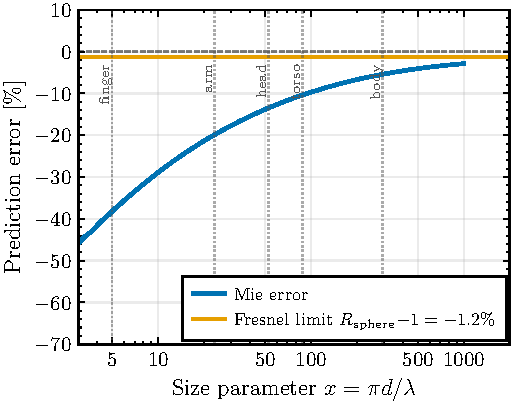
\includegraphics[width=\linewidth]{mie_panel_size.pdf}
    \caption{Across size parameter at $28$~GHz.}
    \label{fig:mie:size}
  \end{subfigure}\hfill
  \begin{subfigure}[t]{0.48\linewidth}
    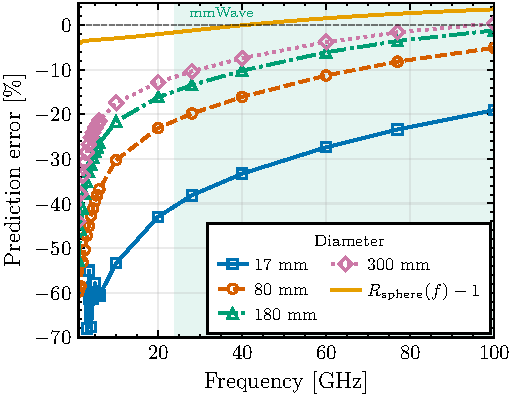
\includegraphics[width=\linewidth]{mie_panel_freq.pdf}
    \caption{Across frequency for four body-part diameters.}
    \label{fig:mie:freq}
  \end{subfigure}
  \caption{Mie validation against lossy spheres with frequency-dependent
  IT'IS skin properties. (a)~Prediction error versus size parameter
  at $28$~GHz. Vertical dashed lines mark body-part sizes. The
  curve converges from below to the Fresnel limit
  $R_{\mathrm{sphere}}-1\approx -1.2\%$ as $x\to\infty$.
  (b)~Prediction error versus frequency for finger ($17$~mm), arm
  ($80$~mm), head ($180$~mm), and torso ($300$~mm) diameters. The
  wireless mmWave band is shaded green. The orange asymptote is
  $R_{\mathrm{sphere}}(f)-1$, the size-independent Fresnel limit.}
  \label{fig:mie}
\end{figure*}

For body-relevant sizes (head, torso) at mmWave, the error is
$0.4\%$ (torso at $100$~GHz) to $14\%$ (head at $28$~GHz), set mostly
by diffraction into the geometric shadow at the low end of the band.
At $28$~GHz the law underestimates absorption, which is a
conservative error in the regulatory sense. For fingers at sub-mmWave frequencies, errors
exceed $30\%$. On body-scale objects in the
claimed regime, the residual is within the dielectric uncertainty on
$T_0$ (\cref{fig:err-budget}). Per-frequency residuals across four
body-part diameters ($17$, $80$, $180$, $300$~mm) are in
Table~\ref{tab:mie-residual} of the SI.

\subsection{Full Fresnel on the Thelonious phantom}\label{subsec:val-fresnel}
The Mie test bounds the Fresnel error on a smooth shape. The phantom
test bounds it on realistic anatomy. We compare the simplified
prediction $\APD^{\mathrm{simp}} = \IPD\,T_0 \pospart{\mu}$ against
the full polarization-aware Fresnel integration $\APD^{\mathrm{full}}
= \IPD\,\Teff(\theta, \mathrm{pol}) \pospart{\mu}$ on the Thelonious
mesh ($23\,826$ triangles, $0.787\,\mathrm{m}^2$ surface area). The
incident plane wave comes from above, with skin properties at
$28$~GHz.

\begin{table}[!t]
\centering
\caption{Geometric law versus full Fresnel integration on the
Thelonious phantom (skin at $28$~GHz, plane wave from above).}
\label{tab:phantom}
\begin{tabular}{lccc}
\toprule
Metric & Simplified & Full Fresnel & Error \\
\midrule
Mean $\APD$ (illum.)     & $0.185$~W/m$^2$ & $0.186$~W/m$^2$ & $0.5\%$ \\
Peak $\APD$              & $0.539$~W/m$^2$ & $0.539$~W/m$^2$ & $0.0\%$ \\
\bottomrule
\end{tabular}
\end{table}

\Cref{tab:phantom} reports the pointwise comparison. For the
$4\,907$ illuminated triangles with
$\theta < 75^\circ$, the local statistics are mean error $-2.6\%$,
root-mean-square $3.2\%$, and range $[-5.3\%, 0.0\%]$. The peak
$\APD$ is recovered exactly because the maximum is at normal incidence,
where $\Teff(0) = T_0$ regardless of polarization. The local error is
below $5.5\%$ everywhere with $\theta < 75^\circ$.
Section~\ref{si:apd-direction} and Fig.~\ref{fig:si-apd-direction}
of the SI extend the analysis to $128$ illumination directions and
three polarization states, and confirm that the per-direction
distribution of total absorbed power clusters around the prediction
$T_0\,\Aperp$ within the directional spread expected from
self-shadowing.

\subsection{Sim4Life FDTD on the Thelonious phantom}\label{subsec:val-fdtd}
The Mie and Fresnel tests check approximations against analytic and
semi-analytic ground truths. Full Sim4Life FDTD on the same
Thelonious mesh, matched dielectric properties, and matched
plane-wave excitation completes the comparison. Two regulatory
metrics are evaluated. The first is the IEC/IEEE~63195 peak $\APD$
averaged over a $4$~cm$^2$ patch. At $7$~GHz on three
lateral and frontal incidence directions with $\theta$-polarization,
the direction-averaged ratio of law to FDTD is $1.027$. Propagating a
$\pm 20\%$ uncertainty on the IT'IS dielectric properties through
the Fresnel coefficient at $7$~GHz gives $\pm 7\%$ on
$T_0$, and the direction-averaged ratio falls inside it. The
per-direction values are $1.06$, $1.20$, and $0.83$. The spread
beyond $\pm 7\%$ reflects FDTD discretization and per-direction
polarization detail in the reference rather than the closed form.

The second metric is the direction-averaged Cauchy formula~\eqref{eq:cauchy-exact}
across $12$ directions and $2$ polarizations at $5.8$~GHz. The ratio
of law to FDTD on direction-averaged total absorbed power is
$1.012$, with $\Aab/A = 0.865$ and $\Tbar(f)$ from \cref{tab:Tbar},
and no fitted parameters. \Cref{fig:val-fdtd} extends the comparison
across $0.45$--$5.8$~GHz.

\begin{figure}[!t]
  \centering
  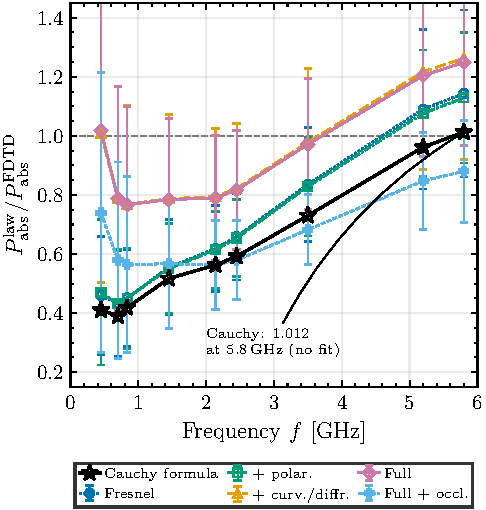
\includegraphics[width=\columnwidth]{fig_kernels_vs_fdtd.pdf}
  \caption{Closed-form prediction versus Sim4Life FDTD on the
  Thelonious phantom. Twelve directions and two polarizations per
  frequency from $0.45$--$5.8$~GHz; error bars show the spread
  across directions. The kernel curves switch on the corrections of
  \cref{sec:corrections} in sequence: ``Fresnel only'' uses
  $T_s/T_p$ at the convex limit, ``+ polarization'' adds the
  polarization-aware $\Teff$, ``+ curvature \& diffraction'' adds
  the $1/(kR)$ refinement, ``Full kernel'' is the constant-$T_0$
  geometric law without occlusion, ``Full + occlusion'' multiplies
  by $\Vis(\rr,\khat)$. The Cauchy stars are the closed-form
  whole-body identity, giving $1.012$ at $5.8$~GHz with no fitted
  % [circa:28e92f05-5978-4a23-aecb-56064194ca27:begin]
  parameters. The layered $\Tlay$ of \cref{subsec:fp} recovers the
  sub-$6$~GHz dip qualitatively.}
  \label{fig:val-fdtd}
\end{figure}

The closed-form Cauchy prediction approaches unity at the upper end
% [circa:28e92f05-5978-4a23-aecb-56064194ca27:begin]
of the band. Below $6$~GHz the surface law underestimates because
% [circa:28e92f05-5978-4a23-aecb-56064194ca27:end]
body-scale Mie and resonance effects do not enter a surface-only law,
in line with the Mie analysis on a sphere of comparable size
parameter.

\subsection{Combined dosimetry literature}\label{subsec:val-waterfall}
\Cref{fig:waterfall} compares the closed-form prediction~\eqref{eq:cauchy-exact} against $168$
volunteers and $5$ FDTD phantoms, reproducing every plateau, dip, and
cross-section scaling reported in the reverberation-chamber and FDTD
literature.

\begin{figure*}[!t]
  \centering
  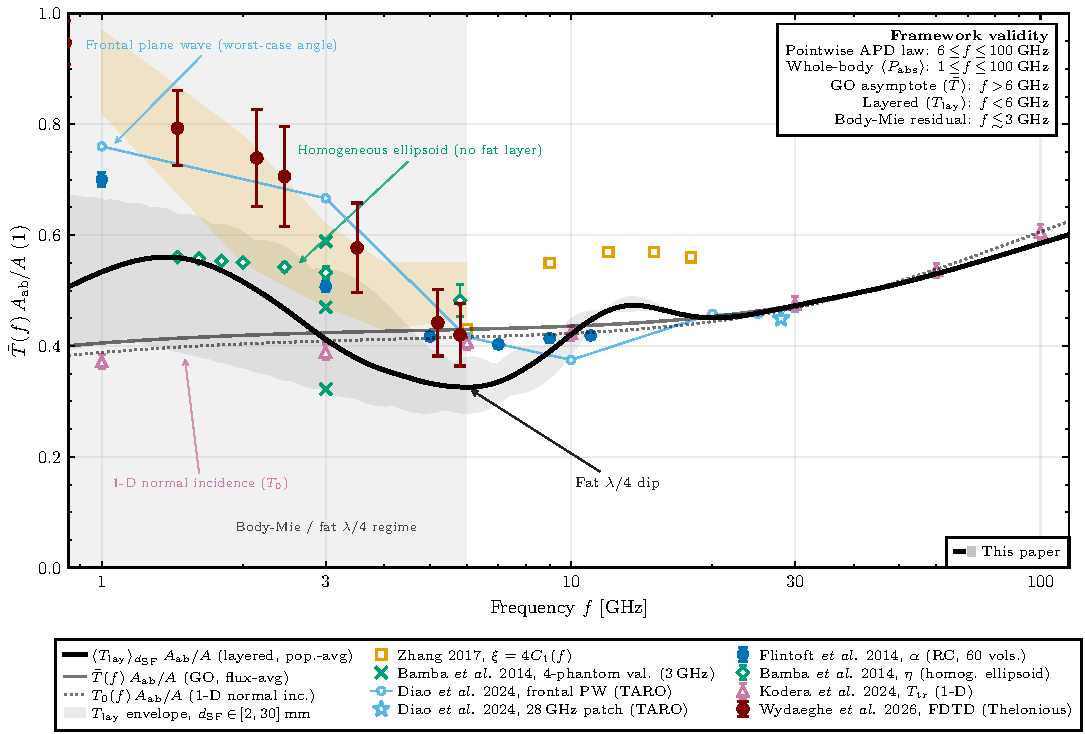
\includegraphics[width=\linewidth]{lit_waterfall_combined.pdf}
  \caption{Closed-form prediction~\eqref{eq:cauchy-exact} compared
  against direction-averaged whole-body absorption ratios in the
  dosimetry literature across $168$ volunteers and $5$ FDTD phantoms
  from $1$ to $100$~GHz. The thick black line is the population-averaged
  layered transmission $\langle\Tlay(f, d_{\mathrm{SF}})\rangle_{d_{\mathrm{SF}}}\,\Aab/A$.
  The average runs over angle of incidence and body-area-weighted
  fat thickness, calibrated to the Flintoft cohort
  (mean $d_{\mathrm{SF}} = 8.5$~mm). The thin black line is the
  geometric-optics asymptote $\Tbar(f)\,\Aab/A$
  from~\eqref{eq:cauchy-exact}. The dotted line is the on-axis
  $T_0(f)\,\Aab/A$, the reference for $1$-D normal-incidence models.
  All three lines converge above $\sim 30$~GHz, where the fat layer
  absorbs the wave and only the air-skin interface remains. The gray
  fill is the $\Tlay$ envelope across $d_{\mathrm{SF}} \in [2, 30]$~mm.
  Dataset conventions: Flintoft $\alpha$ values are linear-regression
  intercepts at $d_{\mathrm{SF}} = 0$ (his Eq.~6, $\gamma_s = 1$).
  Zhang $\xi = 4\,C_1(f)$ uses the Fig.~4.9 plateau ($6$--$18$~GHz)
  plus the Fig.~4.11 envelope ($1$--$6$~GHz). Bamba fits $\eta$ on
  four homogeneous head-tissue ellipsoids, so the data has no
  fat-Fabry-P\'erot feature by construction. Kodera $T_{\mathrm{tr}}$
  is the on-axis Fresnel value for homogeneous skin and tracks the
  dotted reference. Diao back-fits $T_{\mathrm{eff}}$ from a
  single-direction frontal plane wave on TARO at vertical
  polarization, projected area $\mathrm{PA} = 0.54$~m$^2$. Wydaeghe
  FDTD is direction-averaged Sim4Life on Thelonious, $12$ directions
  $\times$ $2$ polarizations per frequency. Error bars are standard
  error of the mean. The inset summarizes the validity regime of the
  framework.}
  \label{fig:waterfall}
\end{figure*}

\Cref{tab:waterfall} states the comparisons numerically. Bamba's
$\eta$ in panel (c) is fit from full-body FDTD on ellipsoidal phantoms
in diffuse-field exposure and absorbs creeping-wave and
finite-curvature contributions that the planar-tissue $\Tbar$ omits;
its convergence to $\Tbar$ at $5.8$~GHz, the upper edge of his
calibration range, is the convergence to the geometric-optics regime
predicted by a Mie analysis of body-scale
spheres~\cite{BohrenHuffman1983}. The $1.45$--$3$~GHz portion of his
fit lies outside the geometric-optics validity window of the present
framework (\cref{tab:bands}); the systematic divergence in panel (c)
below $3$~GHz is the body-Mie regime, not a model failure. Bamba's
anatomical-phantom validation at $3$~GHz returns residuals of
$-39.4\%$, $-11.7\%$, $+10.7\%$, and $+10.6\%$ on the Thelonious,
Billie, Ella, and Duke phantoms (his Table~7). The largest
divergence is on the smallest phantom. The same mechanism appears
in panel (d) on Diao's plane-wave TARO sweep, where
$T_{\mathrm{eff}}$ rises from $0.43$ at $10$~GHz to nearly $0.9$ at
$1$~GHz on the same anatomical phantom~\cite{Diao2024}.

\begin{table*}[!t]
\centering
\caption{Quantitative comparison of the closed-form prediction to the
empirical literature. The shaded sub-$3$~GHz regime, where the
layered tissue model in \cref{subsec:fp} replaces $\Tbar$, is
excluded.}
\label{tab:waterfall}
% [circa:0a267fe8-8ed7-4db9-b221-5873cf61e224:begin]
\begin{tabular}{lp{0.36\linewidth}p{0.26\linewidth}p{0.16\linewidth}}
% [circa:0a267fe8-8ed7-4db9-b221-5873cf61e224:end]
\toprule
Reference & Empirical observation & Closed-form prediction & Match \\
\midrule
Flintoft~\cite{Flintoft2014}
& $\langle Q^a\rangle/\gamma_s = 0.47$--$0.49$ at $7$--$11$~GHz, $60$ volunteers
& $T_0(f) = 0.48$ at $9$~GHz, $\Tbar(f) = 0.50$
& $2\%$--$4\%$ \\
Bamba~\cite{Bamba2014}
& $\eta(f) = 0.48$--$0.56$ at $1.45$--$5.8$~GHz, four FDTD ellipsoids
& $\Tbar(f) = 0.47$--$0.50$
& $3\%$ at $5.8$~GHz; convergent with frequency \\
Zhang~\cite{Zhang2017thesis}
& $\xi = 0.45$--$0.65$ at $6$--$18$~GHz, $48$ subjects
& $\Tbar(f)\cdot\Aab/A = 0.43$--$0.49$
& within scatter \\
Kodera~\cite{Kodera2024}
& $T_{\mathrm{tr}}$ matches $\Aperp$ scaling at $10$--$100$~GHz, parametric FDTD
& $T_{\mathrm{tr}} \equiv T_0$
& $\le 5\%$ \\
Diao~\cite{Diao2024}
& $T = 0.52$ at $28$~GHz, anatomical FDTD
& $T_0 = 0.536$ at $28$~GHz
& $3\%$ \\
Flintoft~\cite{Flintoft2014}
& $-0.0061\,\mathrm{mm}^{-1}$ slope of $\langle Q^a\rangle$ vs $d_{\mathrm{SF}}$ at $3$~GHz
& Layered Fabry--P\'erot in fat
& mechanism, qualitative \\
\bottomrule
\end{tabular}
\end{table*}

Kodera \textit{et~al.}~\cite{Kodera2024} report the closest numerical
counterpart to the present analysis. Their Fig.~13 compiles
whole-body absorbed SAR data over $1$--$10$~GHz at
$\IPD = 10$~W/m$^2$ across nine prior numerical phantom studies and
two reverberation-chamber measurement campaigns; their Fig.~6
extends the same comparison to $1$--$100$~GHz on five parametric
layered models (Models~I--V). The compilation shows the asymptotic
plateau that \eqref{eq:cauchy-exact} predicts. Kodera
\textit{et~al.}\ fit a study-specific $T_{\mathrm{tr}}$ per phantom
and frequency from a one-dimensional multilayer slab calculation;
their homogeneous-skin curve (Fig.~9, right axis) reproduces the
Fresnel $T_0$ within $1$--$2\%$ above $6$~GHz, and oscillates around
that value below $6$~GHz with a multilayer Fabry--P\'erot pattern of
the same form as the layered transmission $\Tlay$ in
\cref{subsec:fp}. \Cref{eq:cauchy-exact} supplies the closed-form
$T_{\mathrm{tr}} \to \Tbar(f)$ that all phantoms converge to in the
geometric-optics regime. The residual phantom-to-phantom spread is
set by the body-shape factor $\Aab/A$.


\section{Higher-order corrections}\label{sec:corrections}

The geometric law~\eqref{eq:geom-law} treats the surface as locally
flat, gates back-facing elements with a sharp $[\cdot]_+$ cutoff, and
ignores power that re-enters the body after a first reflection.
Three systematic corrections refine each of these. The labels in
\cref{fig:val-fdtd} (``Fresnel only,'' ``+ polarization,'' ``+
curvature \& diffraction,'' ``Full kernel,'' ``+ occlusion'') turn
each correction on in turn against the same FDTD reference.

\subsection{Curvature}\label{subsec:corr-curv}
For a surface with twice the local mean curvature $H = 1/R_1 +
1/R_2$, the first-order Physical Optics correction multiplies the
geometric law by $1 + \mu/(kR_1) + \mu/(kR_2)$, where
$k = 2\pi/\lambda$ is the free-space wavenumber. Since
$\pospart{\mu}\cdot\mu = \pospart{\mu}^2$, the per-triangle update
separates additively,
\begin{equation}\label{eq:curv-update}
  \APD^{(j)} = T_0 \sum_i S_i\!\left[
  \pospart{\mu_{ji}} + \frac{H_j}{k}\,\pospart{\mu_{ji}}^2 \right]
  V_{ji}\, ,
\end{equation}
adding a quadratic gate on top of the linear one. The magnitude is
set by $1/(kR)$. \Cref{tab:curv-mag} lists the correction at
$28$~GHz on representative body parts.

\begin{table}[!t]
\centering
\caption{Curvature correction at $28$~GHz ($k \approx 587$~m$^{-1}$).
The correction is below the Fresnel approximation error for most
body regions and concentrates at small features.}
\label{tab:curv-mag}
\begin{tabular}{lccc}
\toprule
Region & $R$\,[mm] & $1/(kR)$ & Correction \\
\midrule
Torso, head & $> 100$ & $< 0.2\%$ & negligible \\
Arm         & approx.\ $40$ & $0.4\%$ & approx.\ $0.4\%$ \\
Finger      & approx.\ $8$  & $2.1\%$ & approx.\ $2\%$ \\
Ear edge    & approx.\ $2$  & $8.5\%$ & approx.\ $8\%$ \\
\bottomrule
\end{tabular}
\end{table}

The correction grows as the wavelength approaches the local
body-part size. At sub-$6$~GHz frequencies the smallest features
have $kR \lesssim 5$ where the correction is no longer small. At
$28$~GHz, only the ear edges and fingertips carry a correction
above the Fresnel error floor.

\subsection{Diffraction at the shadow boundary}\label{subsec:corr-diff}
The sharp $[\cdot]_+$ cutoff at $\mu = 0$ is a geometric-optics
idealization. Diffraction smooths the shadow edge over a Fresnel-zone
width $\sqrt{\lambda R_j}$. The physical activation becomes
\begin{equation}\label{eq:gelu}
  \mu \mapsto \mu\;\tfrac{1}{2}\!\left[1 + \mathrm{erf}(\mu/\sigma_j)\right],
  \qquad \sigma_j = \sqrt{\lambda / (2\pi R_j)}\, .
\end{equation}
The \gls{ICNIRP} centimeter-scale spatial
averaging regularizes the boundary at a length scale larger
than $\sigma_j$ across the wireless band, so the diffraction
correction is significant only for high-resolution local maps or
for comparisons against point measurements. The integrated effect on
whole-body absorbed power on the Thelonious phantom is $1.2\%$ at
$28$~GHz, below $1\%$ above $30$~GHz, and several percent below
$6$~GHz, in line with the Mie analysis on body-scale spheres in
\cref{subsec:val-mie}. Numerical values across $1$--$100$~GHz on
the Thelonious phantom are in Table~\ref{tab:si-diffraction} of the SI.

\subsection{Inter-body reflections}\label{subsec:corr-interbody}
At a surface point the fraction $T_0$ is absorbed and the remaining
$1 - T_0 \approx 0.46$ is reflected. On a nonconvex body, part of
this reflected power re-illuminates another point and contributes
to absorption that the first-bounce law omits. The radiosity series
gives a multiplier $C(\rr) = 1/(1 - \bar{R}\,f(\rr))$ at each point,
where $\bar{R} = 1 - \Tbar \approx 0.46$ is the flux-weighted
reflectance and $f(\rr) \le 1 - \eta(\rr)$ is the recapture fraction
bounded by the local nonvisible hemisphere area.

Two effects keep the body-averaged correction small. First, the bound
$f \le 1 - \eta$ self-compensates: deep concavities ($\eta$ low) have
a high recapture fraction ($f$ high), so the product $\eta\cdot C$
varies much less than $\eta$ alone. Second, specular reflection at
mmWave (skin meets the Rayleigh roughness criterion) reduces $f$ by
roughly a factor of three relative to the diffuse bound. On the
Thelonious phantom at $28$~GHz, the area-weighted recapture fraction is
$f_{\mathrm{global}} \approx 0.09$ under the diffuse bound, giving
$C \approx 1.04$. The specular estimate brings this to
$C \approx 1.01$. The body-averaged correction stays below $2\%$,
smaller than the propagated dielectric uncertainty derived in
\cref{subsec:corr-summary}. The convex-hull energy bound
$\langle P_{\mathrm{abs}}\rangle \le \IPD\,A_{\mathrm{CH}}/4$
(\cref{rem:hull}) brackets the true absorbed power within
$A_{\mathrm{CH}}/A \approx 1.20$ on Thelonious.

\subsection{Error budget}\label{subsec:corr-summary}
\Cref{fig:err-budget} reports two regimes side by side at $28$~GHz on
skin. The worst case is single body part, single direction, pointwise
local. The typical case is whole-body integrated, direction-averaged.
The dielectric input spread is $\pm 20\%$ on $\varepsilon_r$ and
$\sigma$. This is the inter-model gap between Gabriel
1996~\cite{Gabriel1996} and the empirical Gabriel-times-$1.2$ fit
that Christ et al.\ obtained from $S_{11}$ measurements on $37$
volunteers at $40$-$110$~GHz~\cite{Christ2021}, consistent with the
broader spread reported across mmWave measurement
campaigns~\cite{AlekseevZiskin2007,Sasaki2014,Zhadobov2011,Christ2025}.
We evaluate $T_0 = 4n/[(1+n)^2+\kappa^2]$ at the four corners of the
$\pm 20\%$ box. The largest deviation on skin at $28$~GHz is
$\pm 7\%$. The Fresnel approximation worst case is $5.3\%$ pointwise
local (\cref{tab:phantom}). The typical case is $1.2\%$
direction-averaged on whole-body absorbed power (Supplementary
Information, $128$-direction sweep). The diffraction worst case is
$10\%$ on a torso-scale Mie sphere (\cref{subsec:val-mie}). The
typical case is $1.2\%$ integrated on Thelonious (Supplementary
Information, GELU integration). The inter-body reflection worst
case is $4\%$ under the diffuse bound. The typical case is $1\%$
under specular at mmWave (\cref{subsec:corr-interbody}). In the
typical case every model error sits below the dielectric uncertainty.

\begin{figure}[!t]
  \centering
  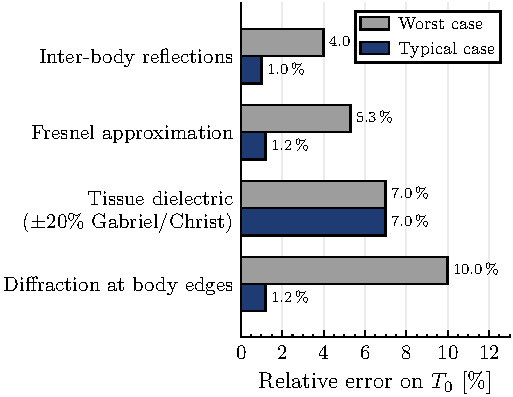
\includegraphics[width=\columnwidth]{error_budget_comprehensive.pdf}
  \caption{Error budget for the geometric law in two regimes at
  $28$~GHz on skin. Worst case is single body part, single direction,
  pointwise. Typical case is whole-body integrated,
  direction-averaged. Only the dielectric uncertainty stays large in
  the typical case.}
  \label{fig:err-budget}
\end{figure}


\section{Compliance and corollaries}\label{sec:compliance}

Regulatory compliance reduces to a function of three precomputed
scalars, with a corollary for the peak spatial-average SAR over a
$10$~g cube.

\subsection{Whole-body SAR threshold}\label{subsec:compl-wb}
The ICNIRP 2020 guidelines~\cite{ICNIRP2020} specify a whole-body
average SAR limit of $0.08$~W/kg for the general public. With
$\mathrm{SAR}_{\mathrm{wb}} = P_{\mathrm{abs}}/m$ and the
direction-resolved bound $D(\khat) = 4\Aperp(\khat)/\Aab \le
2A_{\mathrm{CH}}/\Aab$ on the absorption directivity, the worst-case
threshold is
\begin{equation}\label{eq:Sinc-max-worst}
  \IPD_{\max} = \frac{0.16\,m}{\Tbar\,A}\, ,
\end{equation}
a closed-form function of the body mass $m$, the body surface area
$A$, and the tissue transmission $\Tbar$, none of which requires
an FDTD solve on the specific exposure scenario. The convex-hull
directivity bound $D \le 2 A_{\mathrm{CH}}/\Aab$ together with the
empirical observation $A_{\mathrm{CH}} \approx A/\bar\eta$ on the
human body cancels the ambient-occlusion factor $\bar\eta$ in the
worst-case algebra, leaving $A$ rather than $\Aab$ in the
denominator.

Body surface area follows the Du Bois formula~\cite{DuBois1916} $A
\approx 0.007184\,m^{0.425}\,h^{0.725}$ with mass in kg and height in
cm, so $\IPD_{\max}$ scales as $m/A \propto
\mathrm{BMI}^{0.575}\,h^{0.425}$. \Cref{tab:anthro} evaluates
\eqref{eq:Sinc-max-worst} on a representative population at
$28$~GHz with $\Tbar = 0.543$. The scaling
matches the observation in the dosimetry
literature~\cite{Hirata2007corr,Dimbylow2002} that absorption
cross-section scales with surface area while mass scales with
volume. Section~\ref{si:anthro} of the SI works out the Du Bois
scaling step by step and bounds the linearly polarized worst-case
correction to \eqref{eq:Sinc-max-worst} via the body polarization
directivity.

\begin{remark}[Reference-level shortfall for smaller body sizes]
\label{rem:reflevel-shortfall}
The ICNIRP general-public reference level above $6$~GHz is
$10$~W/m$^2$~\cite{ICNIRP2020}. Reference levels are the
operationally measured incident-power-density limits intended to
imply compliance with the underlying basic restriction (here
$0.08$~W/kg whole-body SAR). \Cref{tab:anthro} shows
$\IPD_{\max} = 6.2$, $7.6$, and $9.9$~W/m$^2$ for the infant,
child, and adolescent rows under the worst-case directional bound
$D \le 2A_{\mathrm{CH}}/\Aab$. The reference level exceeds these
thresholds by $61\%$, $32\%$, and $1\%$, respectively. The closed
form gives certificates of provable basic-restriction
non-compliance for the smaller body sizes at the existing
reference level under worst-case directional exposure.
Under realistic plane-wave or multipath exposure the directivity
is substantially below this worst case, and the basic restriction
is met~\cite{ICNIRP2020}. The closed form makes both the worst-case
and the directional-average evaluation explicit.
\end{remark}

\begin{table}[!t]
\centering
\caption{Worst-case compliance threshold across the human
population at $28$~GHz with $\Tbar = 0.543$. The threshold
varies by a factor of about two between an infant and a large adult.}
\label{tab:anthro}
\small
\setlength{\tabcolsep}{3pt}
\begin{tabular}{lccc}
\toprule
Body type & $m$\,[kg] & $h$\,[cm] & $\IPD_{\max}$\,[W/m$^2$] \\
\midrule
Infant ($1$~yr) & 8   & 70  & 6.2  \\
Child ($6$~yr)  & 20  & 110 & 7.6  \\
Adolescent      & 50  & 160 & 9.9  \\
Adult (ref.)    & 70  & 170 & 11.4 \\
Large adult     & 100 & 180 & 13.5 \\
\bottomrule
\end{tabular}
\end{table}

\subsection{Peak spatial-average SAR over a 10~g cube}
\label{subsec:compl-cube}
ICNIRP retains the peak spatial-average SAR over a $10$~g cube of
tissue as the basic restriction below $6$~GHz, prescribed by
IEC/IEEE~62704~\cite{62704-1} and IEEE~C95.3~\cite{C953}. Above
$6$~GHz the basic restriction switches to \gls{APD} and the cube
quantity is retained only as a sanity
bound~\cite{Hirata2021,Samaras2019}. The closed form takes two
shapes across the $6$~GHz boundary, and we treat the two regimes
in turn. Let $\alpha = k_0\,\mathrm{Im}(\ntilde)$ be the field decay
rate, $L = (m/\rho_m)^{1/3} = 21.5$~mm the cube side at
$\rho_m = 1000$~kg/m$^3$ and $m = 10$~g, and $\delta_{\mathrm{SAR}}
= 1/(2\alpha)$ the SAR penetration depth.

In the thin-skin regime $\alpha L \gg 1$, the volumetric SAR integral
collapses to a surface integral over the body patch inside the cube.
Energy conservation on the axis-aligned cube returns the Cauchy
projection along $\khat$.

\begin{corollary}[Thin-skin cube SAR]\label{cor:cube}
For a body that fills the cube cross-section perpendicular to
$\khat$, the peak spatial-average SAR over an axis-aligned cube of
side $L$ satisfies
\begin{equation}\label{eq:cube}
  \langle\mathrm{SAR}\rangle_{\mathrm{cube}}
  = \frac{\IPD\,T_0}{\rho_m\,L}\,
    \bigl(|k_x| + |k_y| + |k_z|\bigr)\, ,
\end{equation}
exact in the limit $\alpha L \gg 1$.
\end{corollary}

The factor $|k_x| + |k_y| + |k_z|$ equals $1$ along a cube axis and
$\sqrt{3}$ along the space diagonal~\cite{Cauchy1841}. For skin at
$28$~GHz, $\alpha L \approx 45$ and the residual is below
$e^{-90} \approx 10^{-39}$. \Cref{cor:cube} gives the cube quantity
from one scalar multiplication per surface point, against the
iterative voxel-by-voxel cube expansion specified by IEC/IEEE~62704.
\Cref{tab:depth} shows the depth parameter $2\alpha L$ falling from
approximately $90$ at $60$~GHz to approximately $1$ at $0.9$~GHz on
skin. This
marks the boundary at which the thin-skin shortcut breaks down.

\begin{table}[!t]
\centering
\caption{Skin-tissue depth parameter across frequency
($L = 21.5$~mm, IT'IS Cole--Cole). $h(2\alpha L)$ is the fraction of
the surface SAR surviving mass-averaging to depth $L$, and
$C = 1 - e^{-2\alpha L}$ is the capture fraction.}\label{tab:depth}
\small
\begin{tabular}{rcccc}
\toprule
$f$\,[GHz] & $\delta_{\mathrm{SAR}}$\,[mm] & $2\alpha L$ & $h$ & $C$ \\
\midrule
0.9  & 19.9 &  1.1 & 0.61  & 0.67 \\
2.45 & 11.3 &  1.9 & 0.45  & 0.85 \\
5    &  5.3 &  4.1 & 0.24  & 0.98 \\
10   &  1.9 & 11.3 & 0.088 & 1.00 \\
28   & 0.46 & 46.7 & 0.021 & 1.00 \\
60   & 0.24 & 89.9 & 0.011 & 1.00 \\
\bottomrule
\end{tabular}
\end{table}

Below $6$~GHz the depth parameter on fat falls to order unity. The
wave passes through tissue layers without saturating. The field
develops a standing-wave structure with internal reflections. The
thin-skin shortcut overpredicts the cube SAR by up to a factor of
two, and the cube maximum can be below the body surface. A three-layer planar
model (skin $d_1 \approx 2$~mm, fat $d_2 \approx 5$--$20$~mm,
semi-infinite muscle) at normal incidence gives a closed-form cube
SAR via Chew recursion~\cite{Chew1995} of the layer transmission and
reflection coefficients. Section~\ref{si:layered} of the SI gives
the full derivation. Fig.~\ref{fig:si-sar-z} of the SI renders the
standing-wave SAR profile across the canonical stack at $2.45$~GHz.

The layer transmission $\Tlay(f)$ replaces
$T_0$ in the cube formula~\eqref{eq:cube} below $6$~GHz; the
cube-averaged SAR is enhanced over its half-space prediction by a
standing-wave Fabry--P\'erot factor of order $2$--$4$ at fat-resonance
antinodes (\cref{eq:subsurface-criterion}), and the cube maximum
migrates below the surface in fat. Differentiating the standing-wave SAR at $z = 0$ in
skin (SI Eq.~\ref{eq:dSAR-dz-SI}) gives the criterion
\begin{equation}\label{eq:subsurface-criterion}
  |g_1|^2 - \frac{2\beta_1}{\alpha_1}\,|g_1|\sin\psi_1 > 1\, ,
\end{equation}
under which the cube maximum lies below the body surface, where
$g_1 = \widetilde\Gamma_2\,e^{-2 i k_0 \ntilde_1 d_1}$ is the
backward-to-forward amplitude ratio in the skin layer,
$\alpha_1, \beta_1$ are the imaginary and real parts of the skin
wavenumber, and $\psi_1 = \arg g_1$. For a $2$~mm skin / $10$~mm
fat / muscle stack at $2.45$~GHz the criterion evaluates to $7.9$,
well above unity, so the peak is in the fat-muscle stack where
forward and backward waves interfere constructively. Thin lossy skin
over thick low-loss fat over lossy muscle gives a Fabry--P\'erot
enhancement of order $[(1+|g_1|)/(1-|g_1|)]^2$ at antinodes, factors
of $2$--$4$ for typical anatomy.


\section{Discussion}\label{sec:disc}

Equations~\eqref{eq:geom-law} and~\eqref{eq:cauchy-exact} hold
quantitatively above approximately $1$~GHz on whole-body absorbed
power and above approximately $6$~GHz pointwise on the surface, with
documented sub-$6$~GHz behavior from~\eqref{eq:T-lay}. The
low-frequency boundary is set by three independent physical scales:
body opacity, the body-scale Mie regime, and whole-body resonance.
The high-frequency boundary is set by two, the softening of the
pseudo-Brewster compensation and skin surface roughness, both gentler
than the low-frequency boundary.

\subsection{Low-frequency boundary}\label{subsec:disc-lower}

The opacity criterion places the lower validity limit near
$700$~MHz--$1$~GHz for limbs and near $250$~MHz for a torso,
below which the wave passes through the body rather than being fully
absorbed at the surface. The Cauchy identity requires the SAR
penetration depth to be small against body dimensions. The
penetration depth in muscle from the IT'IS Cole--Cole model is
$32$~cm at $100$~MHz, $13$~cm at $300$~MHz, $4$~cm at $1$~GHz,
$1.5$~cm at $3$~GHz, $5$~mm at $6$~GHz, and $0.5$~mm at $28$~GHz.
The opacity criterion $\delta_{\mathrm{SAR}} \ll R_{\mathrm{body}}$
for an arm or leg cross-section ($R \approx 5$~cm) and for a torso
($R \approx 15$~cm) produces these thresholds. Below the limb
threshold the wave reflects from the far air interface, and the
surface-only law breaks down. Section~\ref{si:layered} of the SI
(paragraph ``Where the layered model breaks'') details the three
breakdown regimes: whole-body resonance, finite-thickness anatomy,
and body-traversing multipath.

The Mie regime sets a second lower limit: the surface law
% [circa:28e92f05-5978-4a23-aecb-56064194ca27:begin]
underestimates absorption below $3$--$6$~GHz on a torso and below
% [circa:28e92f05-5978-4a23-aecb-56064194ca27:end]
$1$~GHz on a child phantom, where diffraction into the geometric
shadow contributes $5\%$--$14\%$. The geometric-optics limit
requires $ka \gg 1$ where $a$ is a body characteristic dimension.
For a torso ($a \approx 0.4$~m), $ka = 0.84$ at $100$~MHz, $2.5$
at $300$~MHz, $8.4$ at $1$~GHz, $25$ at $3$~GHz, and $50$ at
$6$~GHz. The geometric-optics asymptote holds with sub-percent Mie
residual once $ka \gtrsim 30$. The Mie validation in
\cref{subsec:val-mie} quantifies this: the error reaches $14\%$ at
body-part sizes at mmWave frequencies and grows above $30\%$ for
fingers below $6$~GHz. The full residual sweep is in
Table~\ref{tab:mie-residual} of the SI.

Whole-body resonance dominates below approximately $300$~MHz, where
the surface law is the wrong starting point. The body acts as a
half-wave dipole peaked near $70$~MHz for a grounded standing adult
and $175$~MHz for ungrounded~\cite{Durney1986}. Internal fields are
dominated by whole-body current distributions, with hot-spots at
ankles, wrists, and the neck where current density is highest.
Hot-spot positions bear no relation to surface absorbed power
density. The surface-to-volume reduction is the wrong physics in
% [circa:a471a26e-d4cc-4b5f-b18f-f8fa19caf44a:begin]
this band: the \gls{ACS} spikes well above the
geometric-optics value
% [circa:a471a26e-d4cc-4b5f-b18f-f8fa19caf44a:end], and the resonance tail extends to
approximately $300$~MHz before becoming negligible against geometric
absorption.

\Cref{tab:bands} summarizes the resulting band stratification.

\begin{table}[!t]
\centering
\caption{Band stratification of~\eqref{eq:cauchy-exact} on a
human-adult body. Quantitative validity covers $1$--$100$~GHz on
whole-body absorbed power, $6$--$100$~GHz pointwise on the
surface.}
\label{tab:bands}
\small
\setlength{\tabcolsep}{4pt}
\begin{tabular}{@{}>{\raggedright\arraybackslash}p{0.18\linewidth}
                  >{\raggedright\arraybackslash}p{0.42\linewidth}
                  >{\raggedright\arraybackslash}p{0.30\linewidth}@{}}
\toprule
Band & Surface law status & Whole-body identity \\
\midrule
below $300$~MHz
  & wrong physics: resonance and hot-spots
  & FDTD required \\
$0.3$--$1$~GHz
  & qualitative, $10\%$--$30\%$ Mie underestimate
  & qualitative, $\Tlay$ recovers the dip \\
$1$--$6$~GHz
  & integrated within $5\%$--$10\%$, local map degrades
  & quantitative, layered correction matters \\
$6$--$100$~GHz
  & quantitative within $3\%$ pointwise
  & quantitative, Brewster compensation sharpest \\
\bottomrule
\end{tabular}
\end{table}

\subsection{High-frequency boundary}\label{subsec:disc-upper}

The pseudo-Brewster compensation softens above $200$--$250$~GHz,
where the Azzam high-index criterion $|\ntilde| > 2.5$ weakens and
worst-case angular variation grows from $5.6\%$ at $28$~GHz to
approximately $10\%$ at $250$~GHz and $15\%$ at $300$~GHz,
comparable to the dielectric uncertainty on $T_0$
(\cref{fig:err-budget}). Skin refractive-index
modulus from IT'IS Cole--Cole is $4.84$ at $28$~GHz, $3.68$ at
$60$~GHz, and $3.01$ at $100$~GHz; extrapolation puts $|\ntilde|$
near $2.5$ around $200$--$250$~GHz, approximately $2.2$ at
$300$~GHz, and $1.8$--$2$ at $1$~THz.

Skin roughness sets an upper limit near $1$~THz, where the
Rayleigh criterion $h\cos\theta/\lambda < 1/8$ is violated on
papillary-ridge-scale features and diffuse scattering becomes the
dominant correction. Skin features are stratified:
stratum-corneum microtexture at $10$--$100\,\mu$m, papillary ridges
at $0.4$--$0.5$~mm spacing, and gross body curvature at
centimeters. Wavelength is $3$~mm at $100$~GHz, $1$~mm at
$300$~GHz, $0.3$~mm at $1$~THz. The Rayleigh criterion is met at
$100$~GHz on ridge-scale features and is marginal at $300$~GHz.

\subsection{Other regime boundaries}\label{subsec:disc-other}

For sources in the reactive near field ($d < \lambda/(2\pi)$, that
is $1.7$~mm at $28$~GHz), evanescent waves and antenna-body
impedance coupling require full-wave simulation. Outside this regime,
the law applies pointwise with spatially varying inputs.

The dielectric properties of biological tissue have been measured to
within approximately $20\%$ at mmWave~\cite{AlekseevZiskin2007}. This input
uncertainty produces $\pm 7\%$ on $T_0$ through the
sublinear propagation derived in \cref{subsec:corr-summary}, and it
dominates the error budget at every operating regime where the
surface law applies.


\section{Conclusion}\label{sec:conc}

The local \gls{APD} on opaque biological tissue reduces
to $\APD(\rr) = \IPD\,T_0\,\Vis(\rr,\khat)\,
\pospart{\nhat\cdot(-\khat)}$, a closed-form expression in the
surface normal, the incidence direction, and the binary
self-shadowing visibility. The collapse rests on a pseudo-Brewster
compensation between TE and TM Fresnel transmissions that puts
biological tissue in the high-index regime described by
Azzam~\cite{Azzam2015} for optical substrates. The unpolarized
transmission stays within $5.6\%$ of its normal-incidence value
$T_0$ over $[0^\circ, 75^\circ]$ at $28$~GHz and within $5\%$
root-mean-square across $0.3$--$100$~GHz on every biological
tissue with $|\ntilde| > 2.5$.

The direction-averaged whole-body absorbed power on any body opaque
at the wavelength is $\langle P_{\mathrm{abs}}\rangle =
\IPD\,\Tbar(f)\,\Aab/4$, a generalized Cauchy formula in which
$\Tbar(f)$ is one Fresnel quadrature against the IT'IS Cole--Cole
data and $\Aab$ is one ambient-occlusion pass over the body mesh.
The fitted transmission coefficient $T_{\mathrm{tr}}$ in the
numerical-dosimetry literature is identified with $T_0$ in the
geometric-optics limit and with $\Tbar(f)$ on the
direction-averaged total. The empirical efficiency $\eta(f)$ in the
reverberation-chamber literature is identified with $\Tbar\Aab/A$.
The $3$~GHz dip in volunteer chamber data is the layered
Fabry--P\'erot resonance in subcutaneous fat, with the slope predicted
by a three-layer transfer-matrix construction. The closed form matches a full Fresnel surface integration on the
Thelonious phantom within $1.2\%$ direction-averaged on total absorbed
power across $128$ illumination directions.

Whole-body ICNIRP compliance no longer requires a per-scenario
full-wave solve. The threshold becomes a closed-form function of
three precomputed scalars: $\Tbar$, $\Aab$, and the body mass $m$.
The five empirical scalars reported by Bamba, Flintoft, Zhang,
Diao, and Kodera reduce to a single closed-form quantity, and the
phantom-to-phantom and volunteer-to-volunteer spread reduces to the
body-shape factor $\Aab/A$, computed once per body on commodity
hardware.

The dosimetry block at the end of any ray tracer is a single
matrix-vector multiply with positive-part gating. The same GPU
primitives that drive real-time rendering apply directly to
real-time exposure assessment, and gradients propagate back through
standard backpropagation. The gate is a ReLU. Diffraction softens
it to the \gls{GELU} activation of transformers~\cite{Hendrycks2016}
(\cref{eq:gelu}).

The closed forms break down below $1$~GHz, where whole-body
resonance dominates and the surface law is the wrong starting point.
They soften above $200$~GHz, where Azzam's high-index criterion
weakens and skin roughness becomes comparable to the wavelength. A
resonance correction below $1$~GHz and a tighter tissue dielectric
catalog above $100$~GHz are natural directions for future work.
Across the intervening band, every published ground truth is matched
within $\pm 7\%$ on $T_0$ propagated from the $\pm 20\%$
dielectric input uncertainty, and a regulatory campaign that takes
weeks of FDTD reduces to one ambient-occlusion pass and one Fresnel
quadrature.


\section*{Acknowledgment}
This work was supported in part by the European Research Council
(ERC) through ATTO: A New Concept for Ultra-high Capacity Wireless
Networks under Grant 695495, and in part by Methusalem through
SHAPE: Next Generation Wireless Networks. The GOLIAT project (5G
expOsure, causaL effects, and rIsk perception through citizen
engAgemenT) has received funding from the European Union's Horizon
Europe research and innovation program under grant agreement
No.~101057262. Views and opinions expressed are however those of
the authors only and do not necessarily reflect those of the
European Union or the European Health and Digital Executive Agency.
Neither the European Union nor the granting authority can be held
responsible for them.


\begin{thebibliography}{10}
\providecommand{\url}[1]{#1}

\bibitem{ICNIRP2020}
International Commission on Non-Ionizing Radiation Protection,
  ``Guidelines for limiting exposure to electromagnetic fields
  (100\,kHz to 300\,GHz),'' \emph{Health Phys.}, vol.~118, no.~5,
  pp.~483--524, May 2020, doi: \doi{10.1097/HP.0000000000001210}.

\bibitem{Kodera2024}
S.~Kodera, K.~Taguchi, Y.~Diao, T.~Kashiwa, and A.~Hirata,
  ``Computation of whole-body average SAR in realistic human models from
  1 to 100\,GHz,'' \emph{IEEE Trans. Microw. Theory Techn.}, vol.~72,
  no.~1, pp.~91--100, Jan. 2024, doi: \doi{10.1109/TMTT.2023.3289562}.

\bibitem{Diao2024}
Y.~Diao, S.~Kodera, K.~Li, and A.~Hirata, ``Assessment of
  whole-body-average SAR for exposure to electromagnetic fields up to
  30\,GHz using a body model with scaled dielectric parameters,''
  \emph{IEEE Trans. Electromagn. Compat.}, vol.~66, no.~5,
  pp.~1351--1360, Oct. 2024, doi: \doi{10.1109/TEMC.2024.3421521}.

\bibitem{Wydaeghe2026}
R.~Wydaeghe, B.~Stroobandt, S.~Gallucci, M.~Parazzini, G.~Tognola,
  J.~Wiart, G.~Vermeeren, M.~Guxens, E.~Tanghe, and W.~Joseph,
  ``Environmental and auto-induced RF-EMF adult and children far-field
  exposure simulations between 450\,MHz and 26\,GHz,''
  \emph{Phys. Med. Biol.}, 2026, under review.

\bibitem{Bamba2014}
A.~Bamba, W.~Joseph, G.~Vermeeren, A.~Thielens, E.~Tanghe, and L.~Martens,
  ``A formula for human average whole-body SAR$_{\mathrm{wb}}$ under diffuse
  fields exposure in the GHz region,'' \emph{Phys. Med. Biol.}, vol.~59,
  no.~23, pp.~7435--7456, Dec. 2014, doi: \doi{10.1088/0031-9155/59/23/7435}.

\bibitem{Zhang2017thesis}
X.~Zhang, ``Accurate wideband measurement of human body absorption cross
  section in a reverberation chamber: A morphological parameters study
  from 1\,GHz to 18\,GHz,'' Ph.D. dissertation, Dept. Electron., Univ.
  York, York, U.K., 2017. [Online]. Available:
  \url{https://etheses.whiterose.ac.uk/19455/}

\bibitem{ZhangRobinson2020}
X.~Zhang, M.~P. Robinson, I.~D. Flintoft, J.~F. Dawson, and S.~Parker,
  ``Morphological study on human body absorption cross section in a
  reverberation chamber from 1\,GHz to 16\,GHz,'' \emph{IEEE Trans.
  Electromagn. Compat.}, vol.~62, no.~2, pp.~330--337, Apr. 2020.

\bibitem{Azzam2015}
R.~M.~A. Azzam, ``High-index dielectric substrates with nearly constant
  reflectance for incident unpolarized or circularly polarized light over
  a wide range of incidence angles,'' \emph{J. Mod. Opt.}, vol.~62,
  no.~10, pp.~811--815, Jun. 2015.

\bibitem{Cauchy1841}
A.-L. Cauchy, ``M\'emoire sur la rectification des courbes et la
  quadrature des surfaces courbes,'' \emph{C. R. Acad. Sci. Paris},
  vol.~13, pp.~1129--1146, 1841.

\bibitem{Zhukov1998}
S.~Zhukov, A.~Iones, and G.~Kronin, ``An ambient light illumination
  model,'' in \emph{Rendering Techniques '98 (Proc. 9th Eurographics
  Workshop Rendering)}, G.~Drettakis and N.~Max, Eds.
  Vienna, Austria: Springer, 1998, pp.~45--56.

\bibitem{Landis2002}
H.~Landis, ``Production-ready global illumination,'' in \emph{ACM
  SIGGRAPH 2002 Course Notes}, vol.~16, San Antonio, TX, USA, Jul. 2002,
  pp.~87--102.

\bibitem{AkenineMoller2018}
T.~Akenine-M{\"o}ller, E.~Haines, and N.~Hoffman, \emph{Real-Time
  Rendering}, 4th~ed. Boca Raton, FL, USA: A K Peters/CRC Press,
  2018.

\bibitem{Flintoft2014}
I.~D. Flintoft, M.~P. Robinson, G.~C.~R. Melia, A.~C. Marvin, and
  J.~F. Dawson, ``Average absorption cross-section of the human body
  measured at 1--12\,GHz in a reverberant chamber: Results of a human
  volunteer study,'' \emph{Phys. Med. Biol.}, vol.~59, no.~13,
  pp.~3297--3317, Jul. 2014, doi: \doi{10.1088/0031-9155/59/13/3297}.

\bibitem{ITISv5}
IT'IS Foundation, ``Tissue properties database V5.0,'' Z\"urich,
  Switzerland, 2024. [Online]. Available:
  \url{https://itis.swiss/virtual-population/tissue-properties/database/}

\bibitem{Gabriel1996}
S.~Gabriel, R.~W. Lau, and C.~Gabriel, ``The dielectric properties of
  biological tissues: III. Parametric models for the dielectric spectrum
  of tissues,'' \emph{Phys. Med. Biol.}, vol.~41, no.~11,
  pp.~2271--2293, Nov. 1996, doi: \doi{10.1088/0031-9155/41/11/003}.

\bibitem{BornWolf1999}
M.~Born and E.~Wolf, \emph{Principles of Optics}, 7th~ed.
  Cambridge, U.K.: Cambridge Univ. Press, 1999.

\bibitem{Potter1970}
R.~F. Potter, ``Pseudo-Brewster angle and the optical constants,''
  \emph{Appl. Opt.}, vol.~9, no.~7, p.~1717, Jul. 1970.

\bibitem{Ohman1977}
G.~P. Ohman, ``The pseudo-Brewster angle,'' \emph{IEEE Trans. Antennas
  Propag.}, vol.~25, no.~6, pp.~903--904, Nov. 1977.

\bibitem{Funahashi2018}
D.~Funahashi, A.~Hirata, S.~Kodera, and K.~R. Foster, ``Area-averaged
  transmitted power density at skin surface as metric to estimate
  surface temperature elevation,'' \emph{IEEE Access}, vol.~6,
  pp.~77\,665--77\,674, 2018,
  doi: \doi{10.1109/ACCESS.2018.2883733}.

\bibitem{AlekseevZiskin2007}
S.~I. Alekseev and M.~C. Ziskin, ``Human skin permittivity determined
  by millimeter wave reflection measurements,''
  \emph{Bioelectromagnetics}, vol.~28, no.~5, pp.~331--339, Jul. 2007,
  doi: \doi{10.1002/bem.20308}.

\bibitem{Christ2021}
A.~Christ, A.~Aeschbacher, F.~Rouholahnejad, T.~Samaras, B.~Tarigan,
  and N.~Kuster, ``Reflection properties of the human skin from 40 to
  110 GHz: A confirmation study,'' \emph{Bioelectromagnetics},
  vol.~42, no.~7, pp.~562--574, Oct. 2021,
  doi: \doi{10.1002/bem.22362}.

\bibitem{Sasaki2014}
K.~Sasaki, K.~Wake, and S.~Watanabe, ``Measurement of the dielectric
  properties of the epidermis and dermis at frequencies from 0.5~GHz
  to 110~GHz,'' \emph{Phys.\ Med.\ Biol.}, vol.~59, no.~16,
  pp.~4739--4747, Aug. 2014,
  doi: \doi{10.1088/0031-9155/59/16/4739}.

\bibitem{Zhadobov2011}
M.~Zhadobov, N.~Chahat, R.~Sauleau, C.~Le~Quement, and Y.~Le~Drean,
  ``Millimeter-wave interactions with the human body: state of
  knowledge and recent advances,'' \emph{Int.\ J.\ Microw.\ Wirel.\
  Technol.}, vol.~3, no.~2, pp.~237--247, Apr. 2011,
  doi: \doi{10.1017/S1759078711000122}.

\bibitem{Christ2025}
A.~Christ et al., ``Human skin model from 15~GHz to 110~GHz,''
  \emph{Bioelectromagnetics}, vol.~46, no.~7, art.~e70025, 2025,
  doi: \doi{10.1002/bem.70025}.

\bibitem{Hendrycks2016}
D.~Hendrycks and K.~Gimpel, ``Gaussian error linear units (GELUs),''
  Jun. 2016. [Online]. Available: \url{https://arxiv.org/abs/1606.08415}

\bibitem{SionnaRT}
J.~Hoydis, F.~A\"{i}t~Aoudia, S.~Cammerer, M.~Nimier-David, N.~Binder,
  G.~Marcus, and A.~Keller, ``Sionna RT: Differentiable ray tracing for
  radio propagation modeling,'' Mar. 2023. [Online]. Available:
  \url{https://arxiv.org/abs/2303.11103}

\bibitem{Tomita1999}
H.~Tomita, T.~Tagawa, and T.~Wagai, ``Comparison of formulae for
  measuring body surface area in Japanese subjects,'' \emph{J. Tokyo
  Med. Univ.}, vol.~57, pp.~519--527, 1999.

\bibitem{Chew1995}
W.~C. Chew, \emph{Waves and Fields in Inhomogeneous Media}.
  New York, NY, USA: IEEE Press, 1995.

\bibitem{BohrenHuffman1983}
C.~F. Bohren and D.~R. Huffman, \emph{Absorption and Scattering of
  Light by Small Particles}.
  New York, NY, USA: Wiley, 1983.

\bibitem{DuBois1916}
D.~Du~Bois and E.~F. Du~Bois, ``Clinical calorimetry: Tenth paper.
  A formula to estimate the approximate surface area if height and
  weight be known,'' \emph{Arch. Intern. Med.}, vol.~17, no.~6,
  pp.~863--871, Jun. 1916,
  doi: \doi{10.1001/archinte.1916.00080130010002}.

\bibitem{Hirata2007corr}
A.~Hirata, Y.~Nagaya, O.~Fujiwara, T.~Nagaoka, and S.~Watanabe,
  ``Correlation between absorption cross section and body surface area
  of human for far-field exposure at GHz bands,'' in \emph{Proc. IEEE
  Int. Symp. Electromagn. Compat. (EMC)}, Honolulu, HI, USA, Jul. 2007,
  pp.~1--4.

\bibitem{Dimbylow2002}
P.~J. Dimbylow, ``Fine resolution calculations of SAR in the human body
  for frequencies up to 3\,GHz,'' \emph{Phys. Med. Biol.}, vol.~47,
  no.~16, pp.~2835--2846, Aug. 2002,
  doi: \doi{10.1088/0031-9155/47/16/301}.

\bibitem{62704-1}
\emph{Determining the Peak Spatial-Average Specific Absorption Rate
  (SAR) in the Human Body From Wireless Communications Devices, 30\,MHz
  to 6\,GHz--Part 1: General Requirements for Using the
  Finite-Difference Time-Domain (FDTD) Method for SAR Calculations},
  IEC/IEEE Standard 62704-1-2017, 2017.

\bibitem{C953}
\emph{IEEE Recommended Practice for Measurements and Computations of
  Electric, Magnetic, and Electromagnetic Fields With Respect to Human
  Exposure to Such Fields, 0\,Hz to 300\,GHz}, IEEE Standard C95.3-2021,
  2021.

\bibitem{Hirata2021}
A.~Hirata, S.~Kodera, K.~Sasaki, J.~Gomez-Tames, I.~Laakso, A.~Wood,
  S.~Watanabe, and K.~R. Foster, ``Human exposure to radiofrequency
  energy above 6\,GHz: review of computational dosimetry studies,''
  \emph{Phys. Med. Biol.}, vol.~66, no.~8, Apr. 2021, Art. no. 08TR01,
  doi: \doi{10.1088/1361-6560/abf1b7}.

\bibitem{Samaras2019}
T.~Samaras and N.~Kuster, ``Theoretical evaluation of the power
  transmitted to the body as a function of angle of incidence and
  polarization at frequencies ${>}$6\,GHz and its relevance for
  standardization,'' \emph{Bioelectromagnetics}, vol.~40, no.~2,
  pp.~136--139, Feb. 2019.

\bibitem{Durney1986}
C.~H. Durney, H.~Massoudi, and M.~F. Iskander, \emph{Radiofrequency
  Radiation Dosimetry Handbook}, 4th~ed. Brooks Air Force Base,
  TX, USA: USAFSAM, 1986, USAFSAM-TR-85-73.

\end{thebibliography}


\vspace{6pt}

\iffalse
\begin{IEEEbiography}[{\includegraphics[width=1in,height=1.25in,clip,keepaspectratio]{robin.png}}]{Robin Wydaeghe}
received the B.Sc.\ and M.Sc.\ degrees in engineering physics from
Ghent University, Ghent, Belgium, in 2019 and 2021, respectively.
He is currently pursuing the Ph.D.\ degree in engineering physics
with Ghent University. His research interests include computational
electrodynamics, numerical assessment of human electromagnetic field
exposure, and propagation modeling of next-generation wireless
networks.
\end{IEEEbiography}

\begin{IEEEbiography}[{\includegraphics[width=1in,height=1.25in,clip,keepaspectratio]{luc.png}}]{Luc Martens}~(Member, IEEE)
received the M.Sc.\ degree in electrical engineering from Ghent
University, Ghent, Belgium, in 1986, and the Ph.D.\ degree in 1990.
From September 1986 to December 1990, he was a Research Assistant
with the Department of Information Technology (INTEC), Ghent
University. During this period, his scientific work focused on the
physical aspects of hyperthermic cancer therapy. His research dealt
with electromagnetic and thermal modeling and the development of
measurement systems for that application. Since 1991, he has managed
the WAVES research group (formerly the Wireless and Cable Research
Group), INTEC. This group has been part of the IMEC Institute since
2004. Since April 1993, he has been a Professor with Ghent
University. He has authored or coauthored more than 300 publications
in the domain of electromagnetic channel predictions, dosimetry,
exposure systems and health, and wireless communications. His
research interests include modeling and measurement of
electromagnetic channels, electromagnetic exposure (e.g., around
telecommunication networks and cellular base station antennas), and
energy consumption of wireless networks.
\end{IEEEbiography}

\begin{IEEEbiography}[{\includegraphics[width=1in,height=1.25in,clip,keepaspectratio]{gunter.png}}]{G\"unter Vermeeren}~(Member, IEEE)
received the M.Sc.\ degree in industrial engineering from the
KAHO Sint-Lieven, Ghent, Belgium, in July 1998, and the M.Sc.\
degree in electrical engineering and the Ph.D.\ degree in
electrotechnical engineering from Ghent University, Belgium, in
July 2001 and August 2013, respectively. From September 2001 to
September 2002, he joined the Research and Development Department
of network integrator Telindus, Leuven, Belgium. Since September
2002, he has been a Research Engineer with the WAVES research group
in the Department of Information Technology, Ghent University. His
research interests include the numerical modeling and measurement
of electromagnetic radiation in the domain of radio-frequency
dosimetry, electromagnetic exposure, on-body propagation,
interference in communication networks, and medical imaging
systems, including hybrid MRI systems.
\end{IEEEbiography}

\begin{IEEEbiography}[{\includegraphics[width=1in,height=1.25in,clip,keepaspectratio]{emmeric.png}}]{Emmeric Tanghe}~(Member, IEEE)
was born in Tielt, Belgium, in 1982. He received the M.Sc.\ and
Ph.D.\ degrees in electrical engineering from Ghent University,
Ghent, Belgium, in 2005 and 2011, respectively. From 2005 to 2011,
he was a Research Assistant with the Department of Information
Technology, Ghent University -- imec. His scientific research
focused on the modeling of indoor and outdoor propagation through
field measurements. In 2015, he became a Part-Time Professor in
medical applications of electromagnetic fields in and around the
human body. Since 2011, he has been a Postdoctoral Researcher with
Ghent University -- imec, where he focuses on propagation
modeling. From 2012 to 2018, he was a Postdoctoral Fellow of
FWO-V (Research Foundation -- Flanders).
\end{IEEEbiography}

\begin{IEEEbiography}[{\includegraphics[width=1in,height=1.25in,clip,keepaspectratio]{wout.png}}]{Wout Joseph}~(Senior Member, IEEE)
was born in Ostend, Belgium, in October 1977. He received the M.Sc.\
degree in electrical engineering from Ghent University, Ghent,
Belgium, in 2000, and the Ph.D.\ degree in electrical engineering
from Ghent University, Ghent, in 2005. From September 2000 to
March 2005, he was a Research Assistant with the Department of
Information Technology (INTEC), Ghent University. During this
period, his scientific work focused on electromagnetic exposure
assessment. Since April 2005, he has been a Post-Doctoral Researcher
with imec -- UGent / INTEC. From October 2007 to October 2013, he
was a Post-Doctoral Fellow of FWO-V (Research Foundation --
Flanders). Since October 2009, he has been a Professor in the domain
of experimental characterization of wireless communication systems.
His research interests include measuring and modeling
electromagnetic fields around base stations for mobile
communications, health effects of exposure to electromagnetic
radiation, electromagnetic exposure assessment, propagation for
wireless communication systems, and antennas and calibration. He
also specializes in wireless performance analysis and quality of
experience.
\end{IEEEbiography}
\fi


\end{document}
